%!TEX root = ../paper.tex

\section{Web Browsing} \label{label:web}
%\begin{figure*}[t]
%     \subfloat[Clock vs. PLT]{%
%       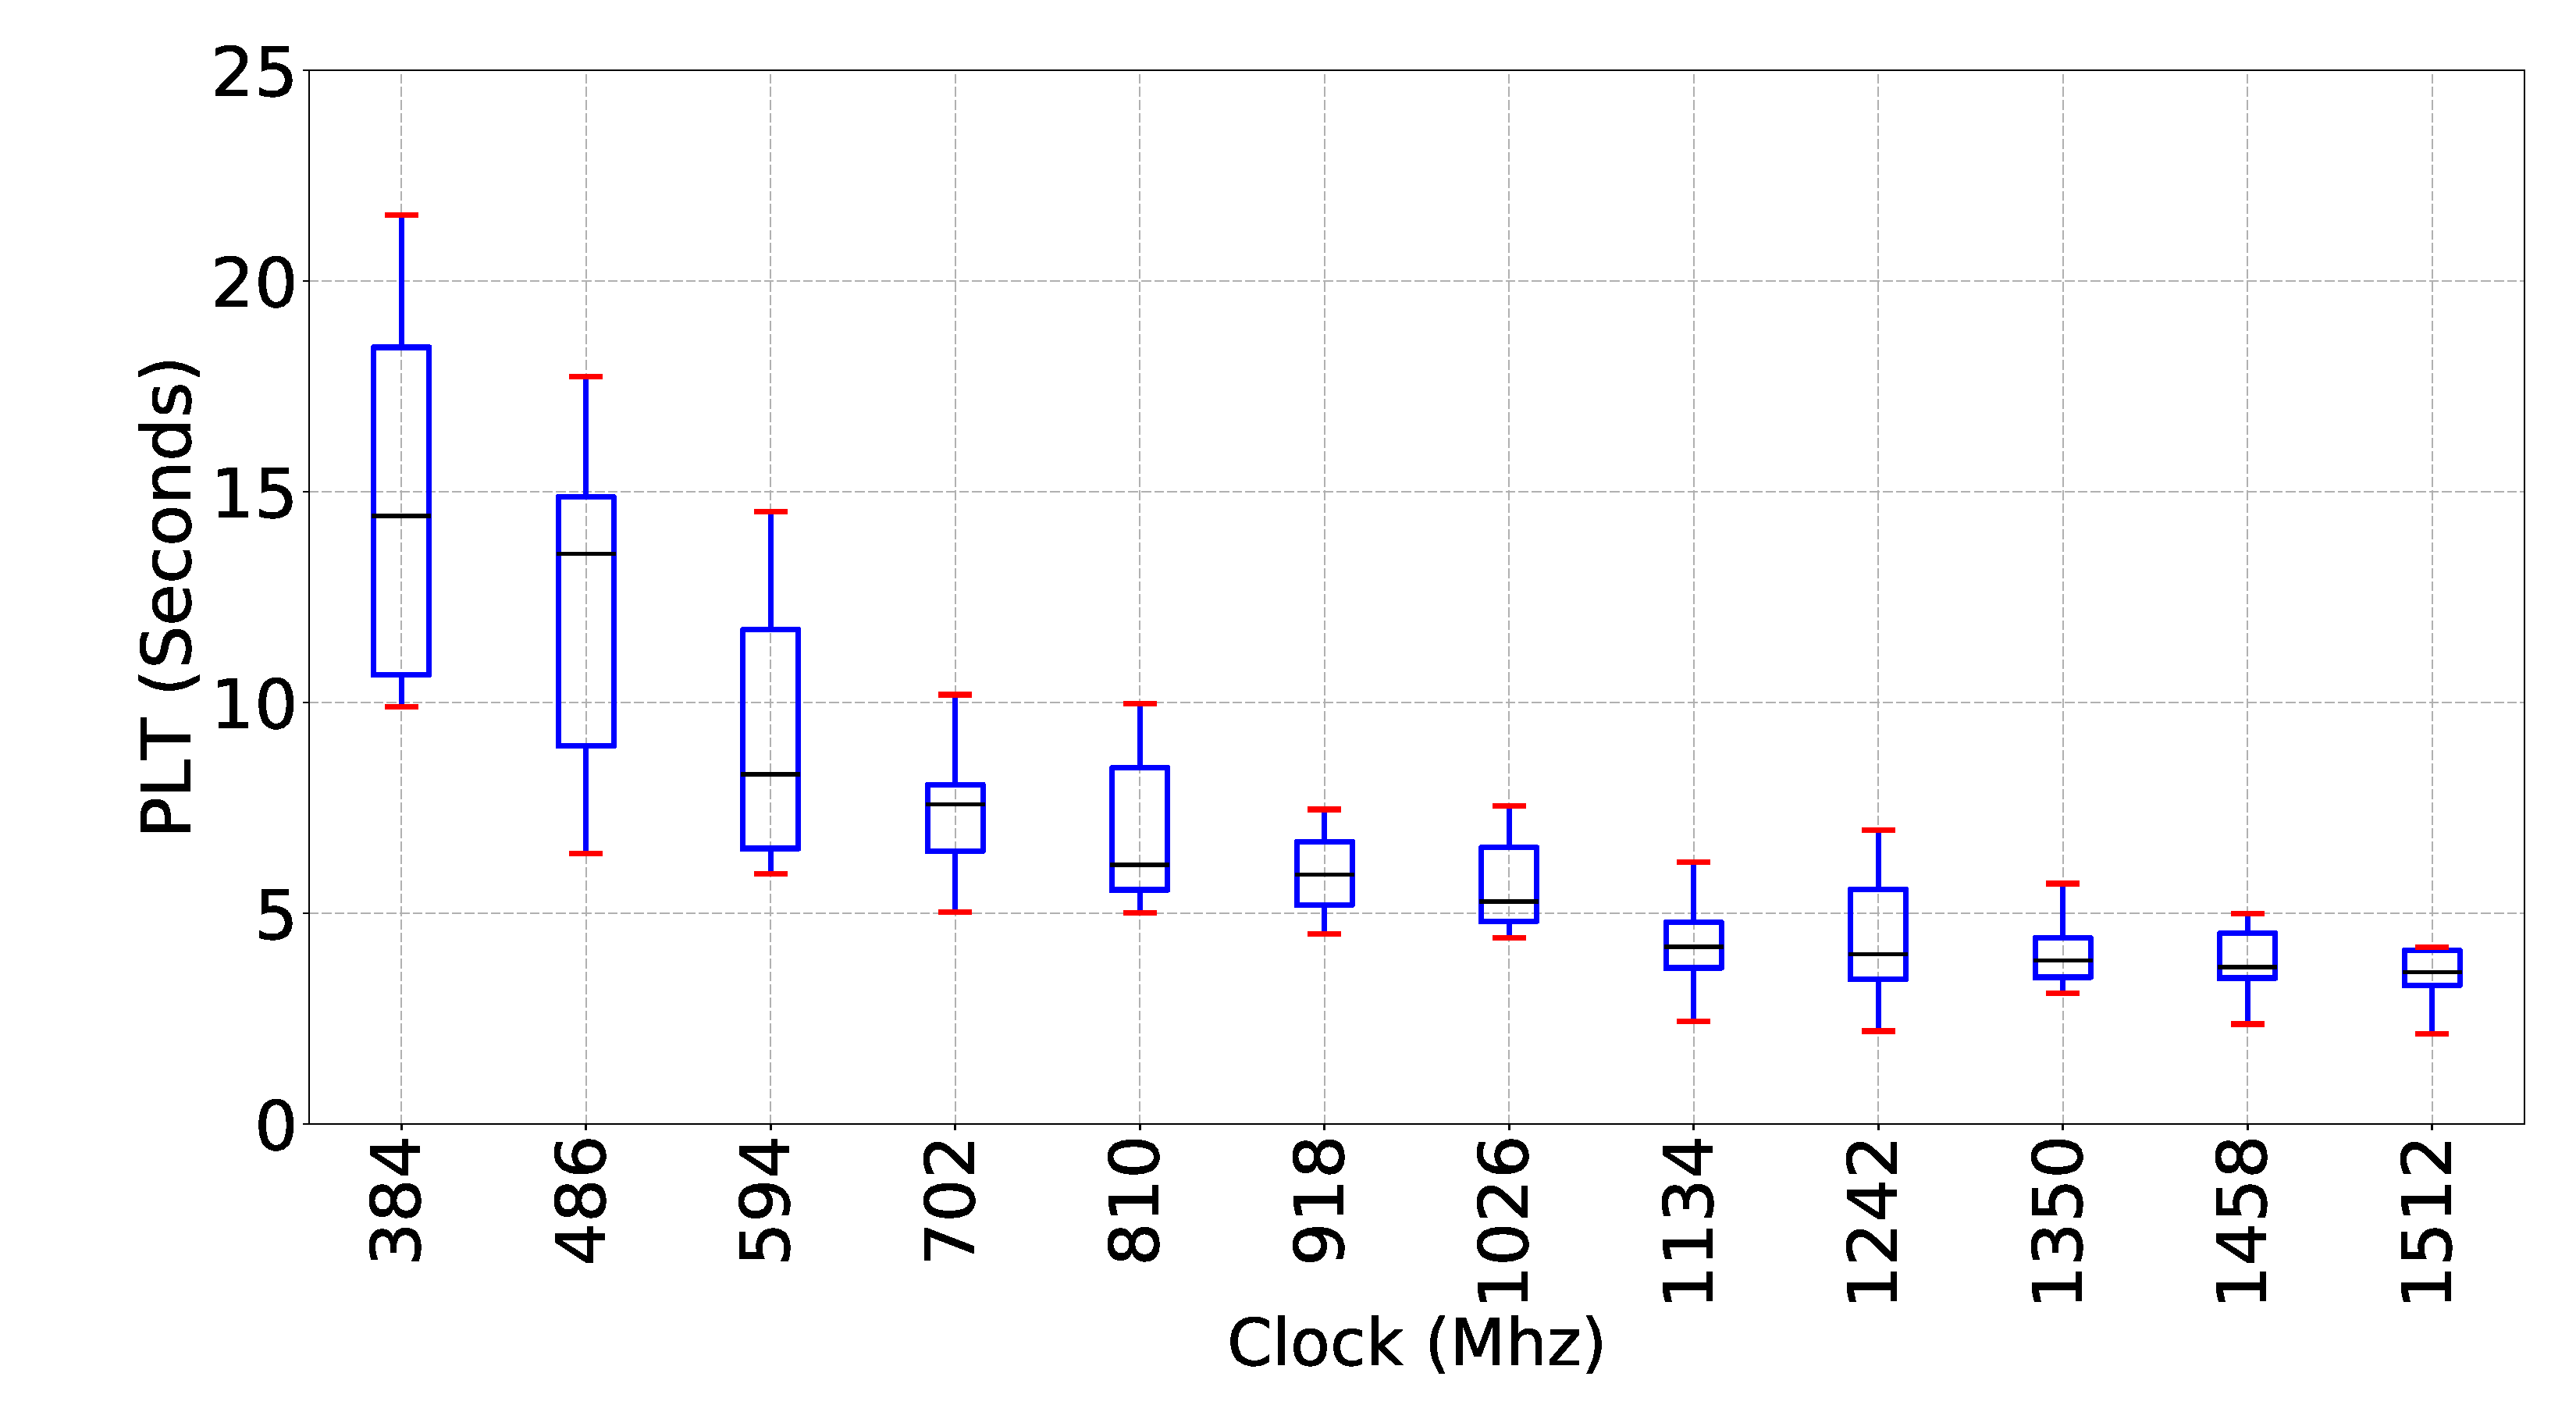
\includegraphics[width=0.5\textwidth]{sections/plt-clock}
%     }
%     \subfloat[Load vs. PLT]{%
%       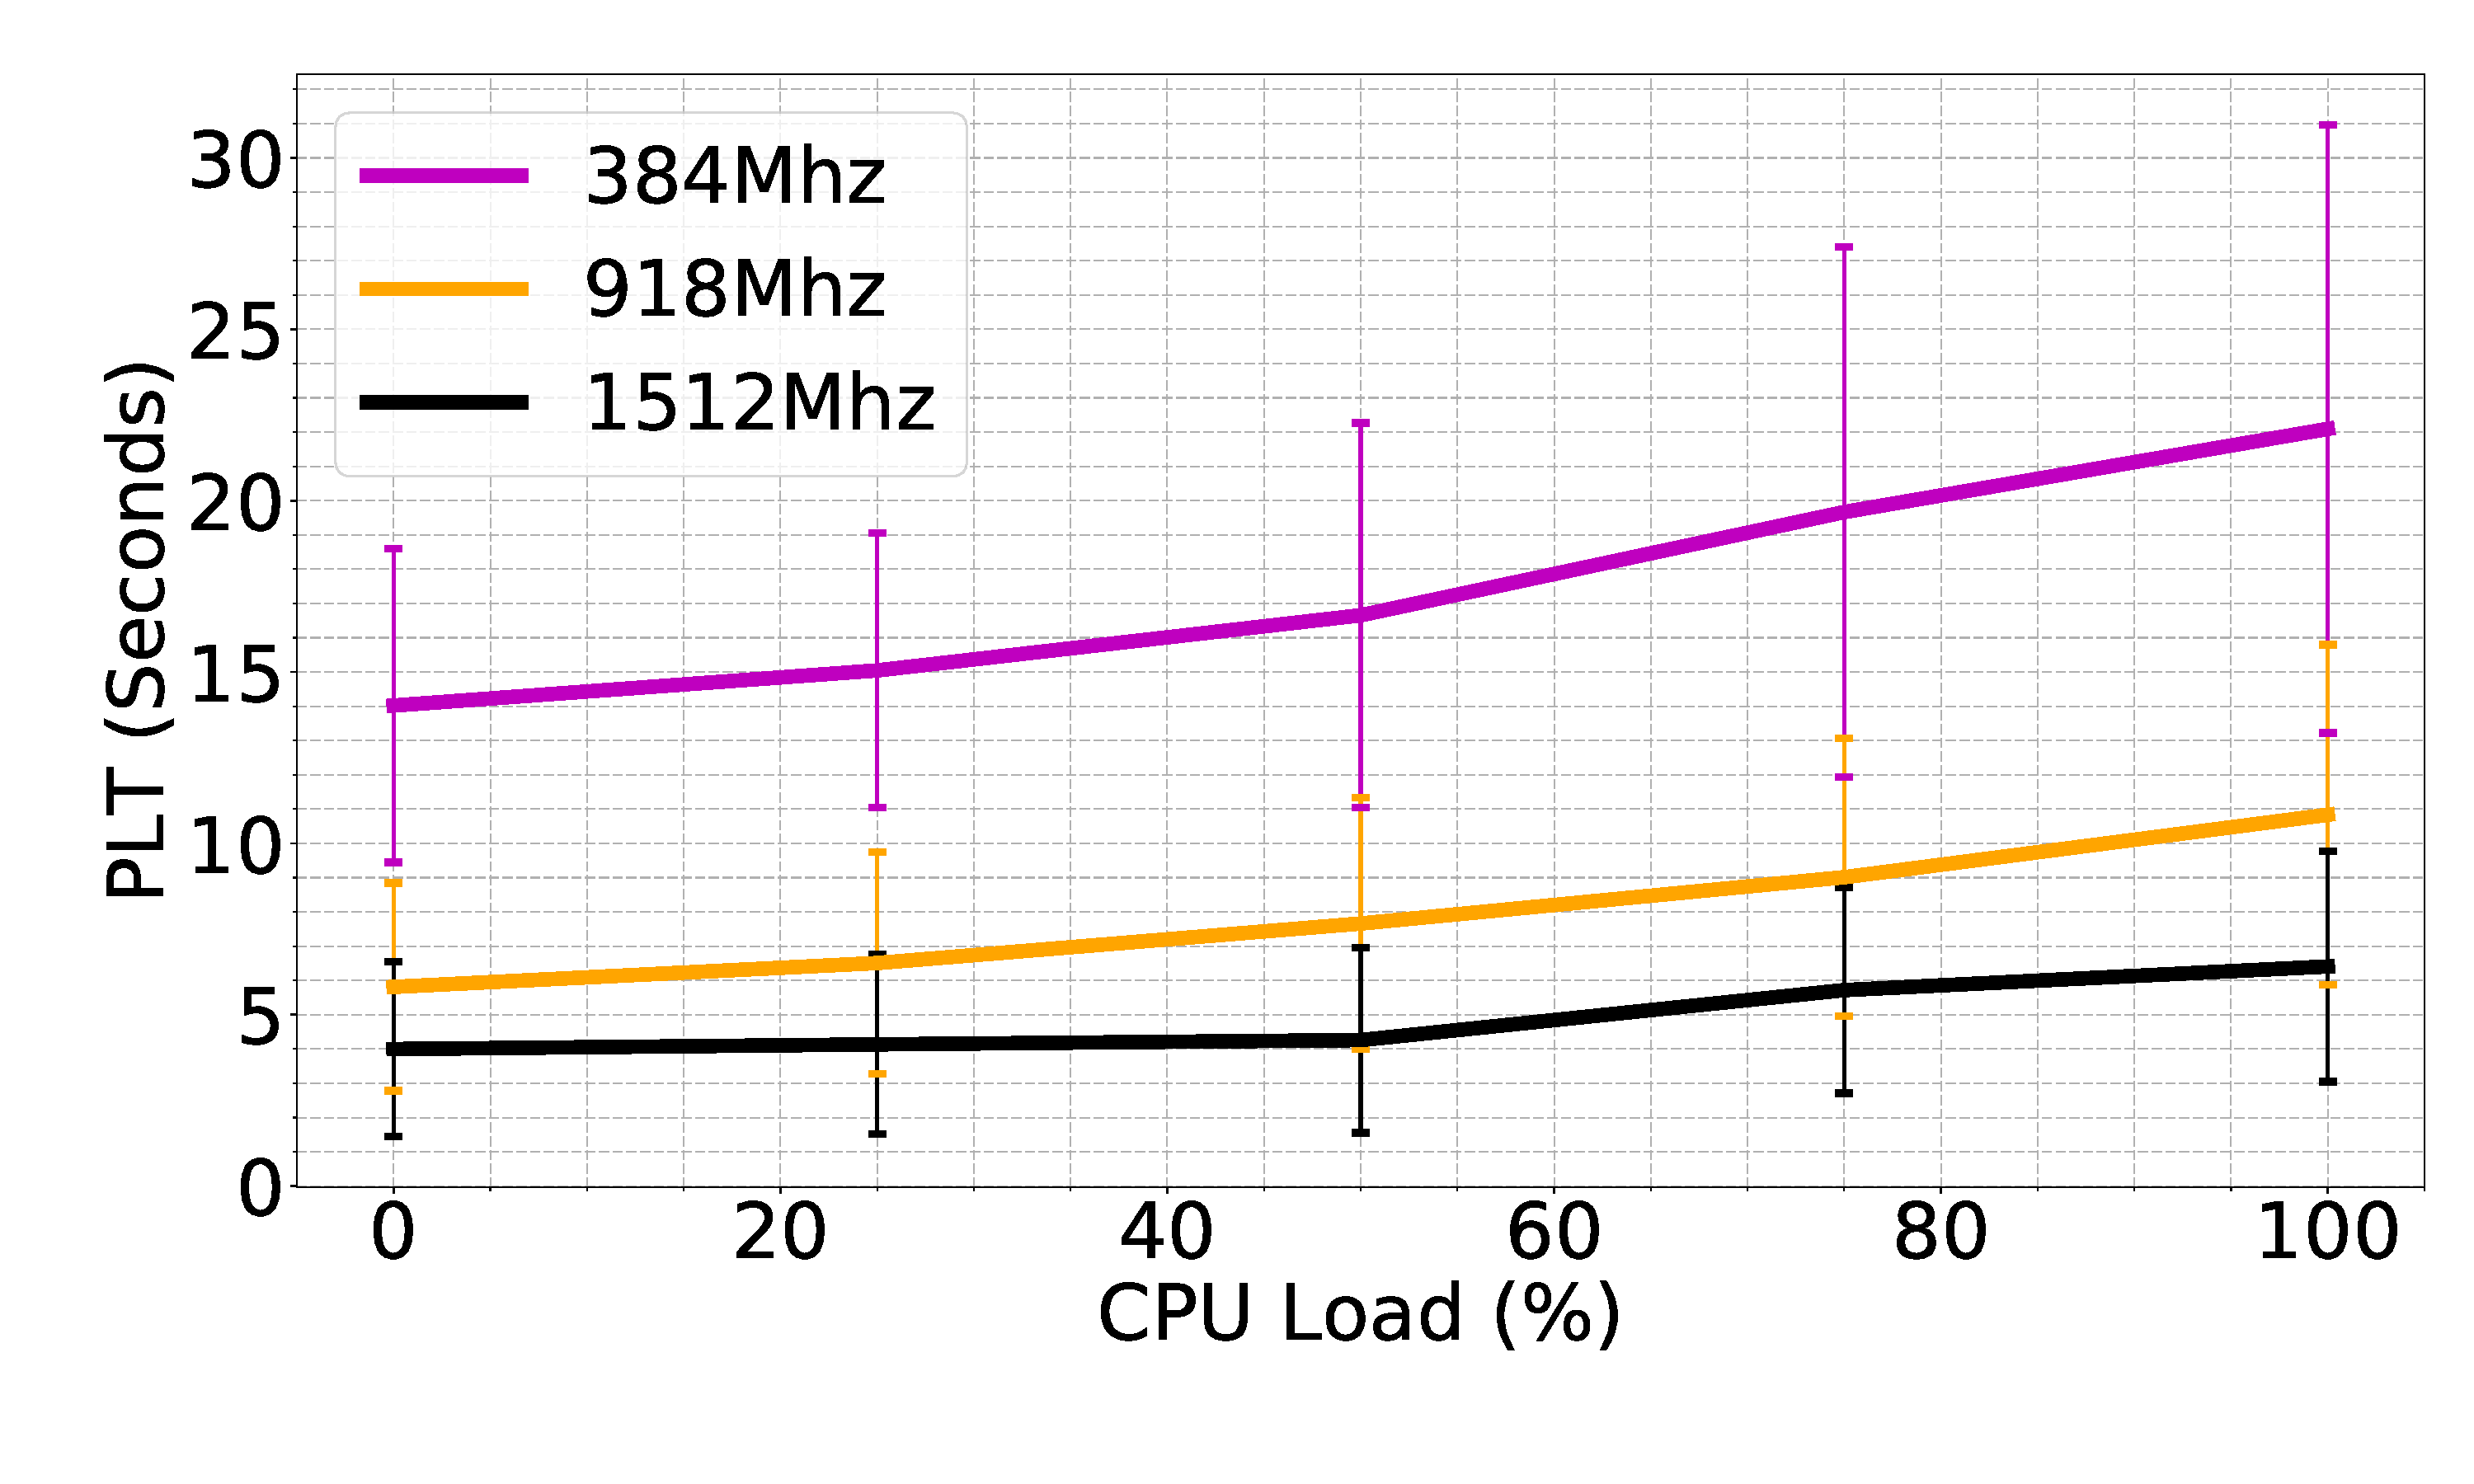
\includegraphics[width=0.5\textwidth]{sections/plt-load}
%     }
%     \caption{\textit{Effect of clock frequency and load on PLT: a) A linear increase from high to low clock (superlinear increase at 486-384Mhz). b) A linear increase till 50\% then after exponential increase.}}
%     \label{fig:clocknload}
%\end{figure*}

\begin{figure}[t]
  \centering
  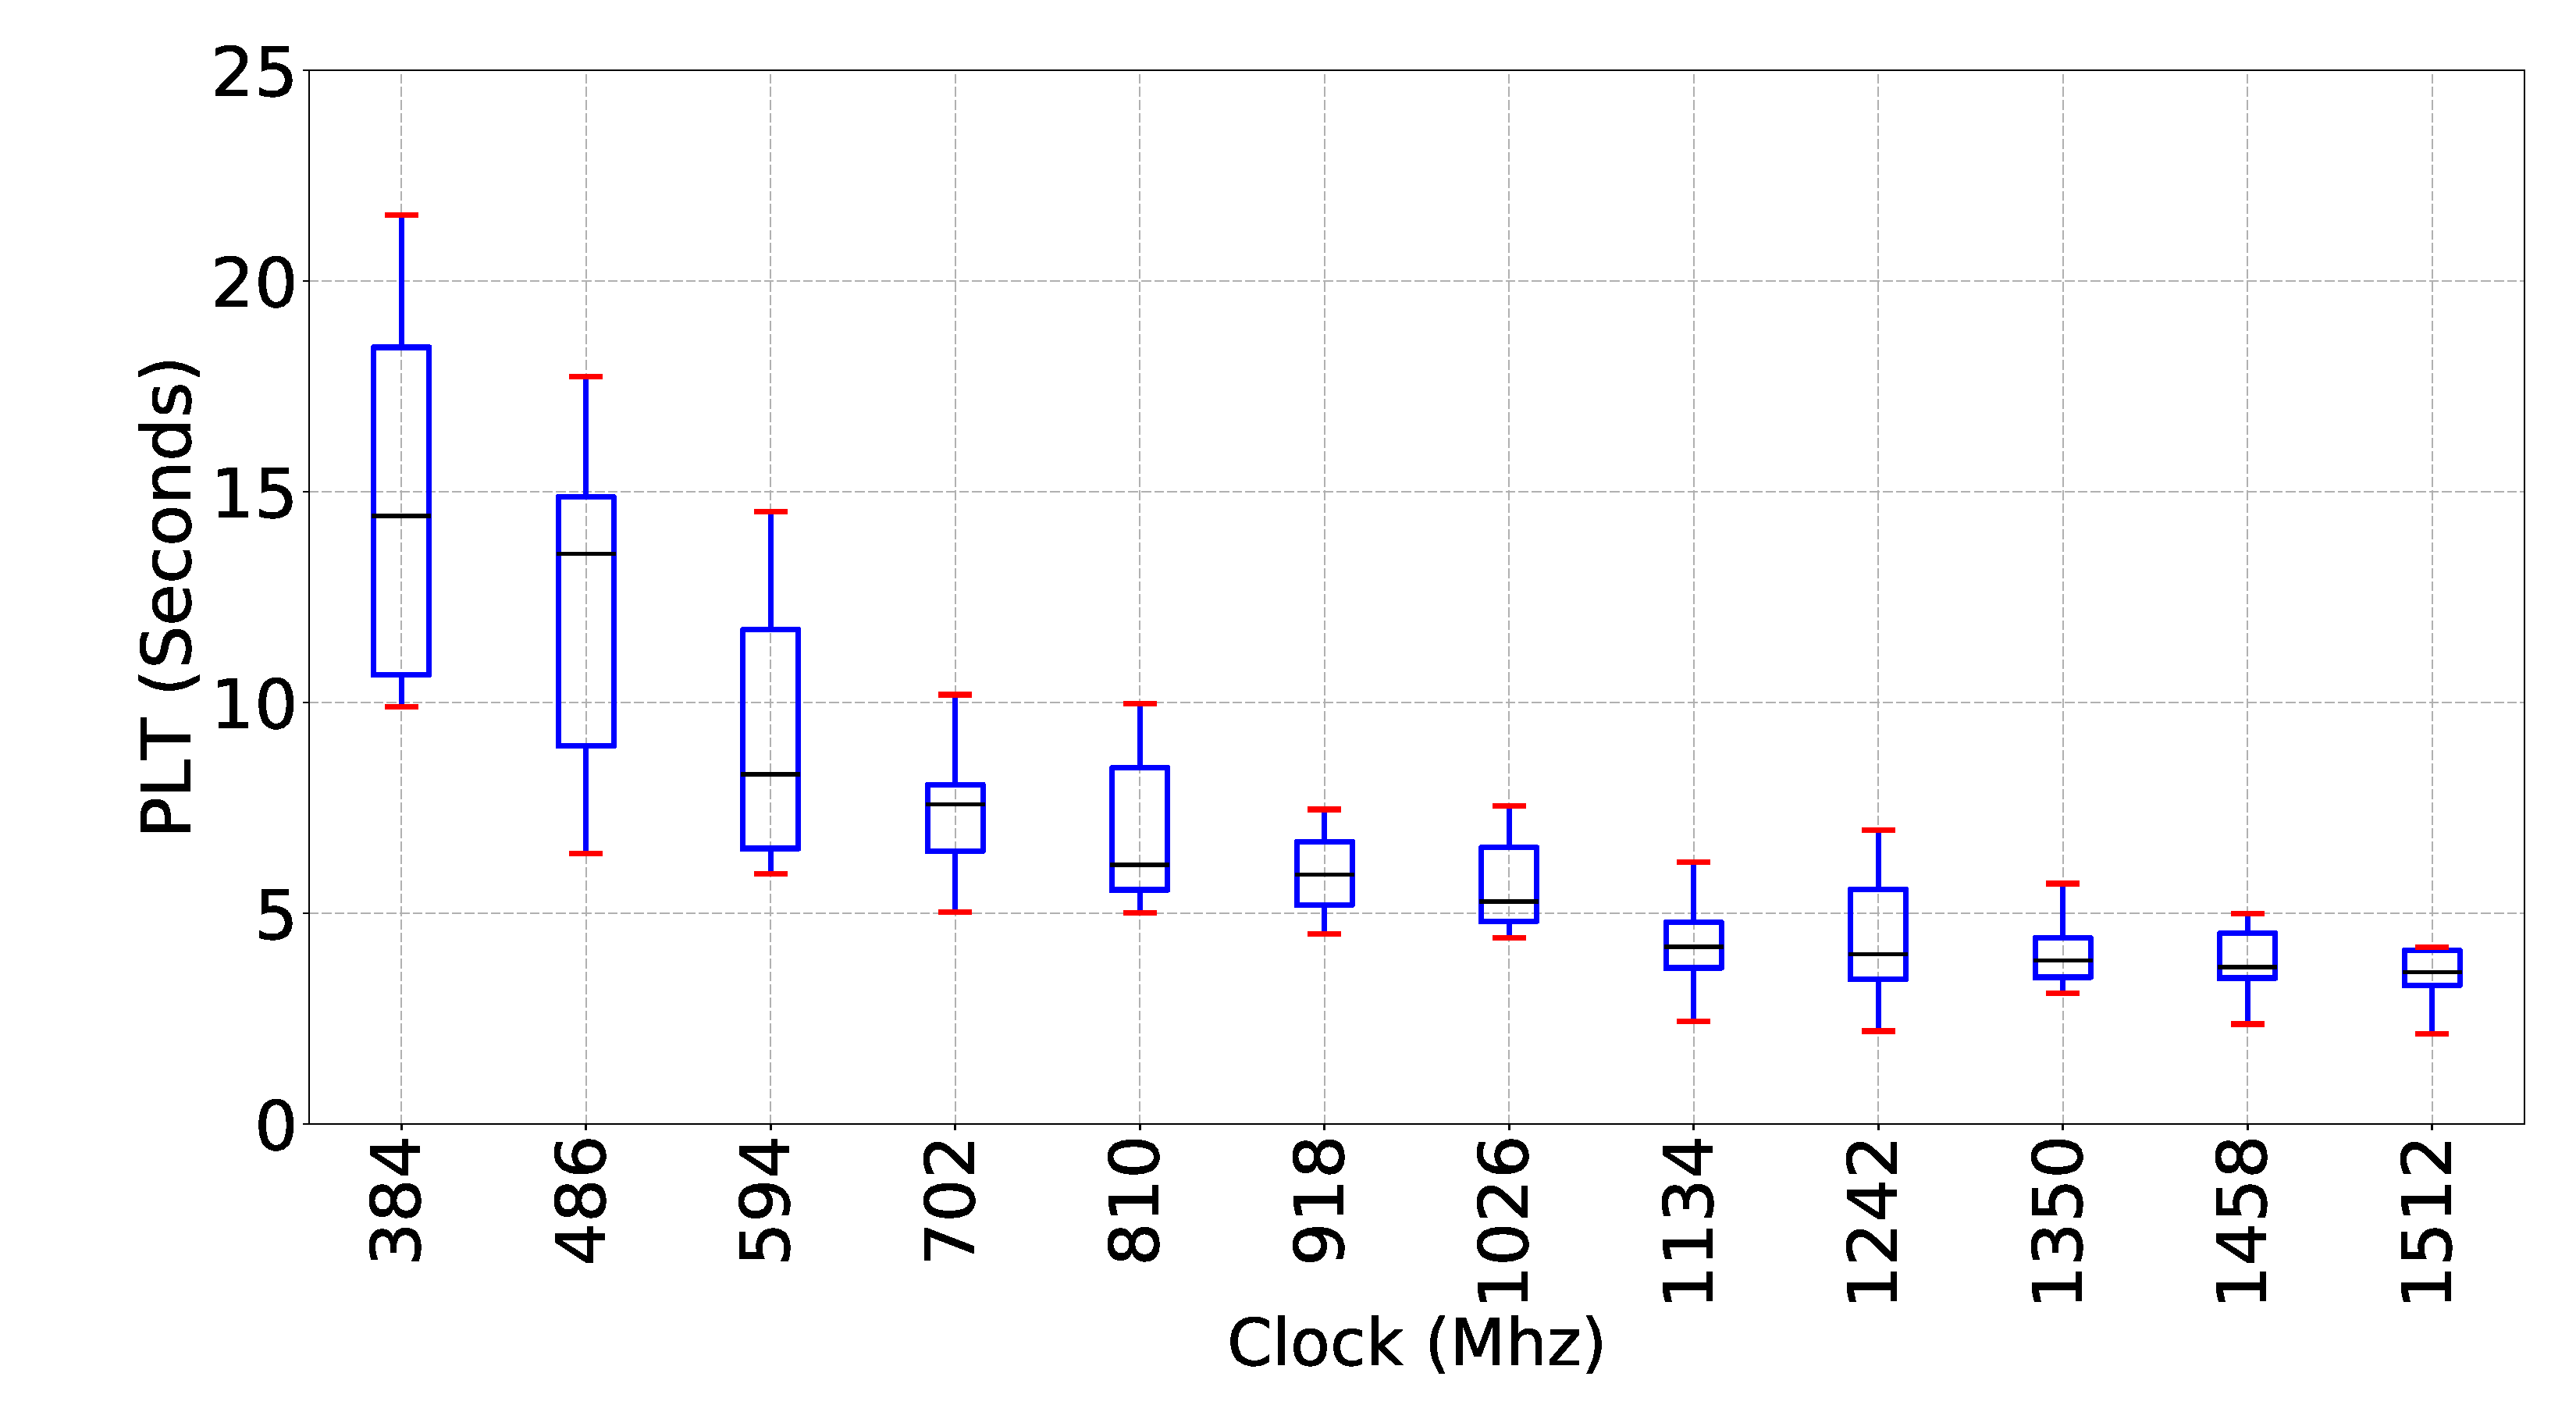
\includegraphics[width=0.9\linewidth]{sections/plt-clock}
    \caption{Web QoE: The average Page Load Time (PLT) across 12 different CPU speeds on Nexus 4. As the CPU speed decreases, PLT increases significantly. }
  \label{fig:plt_clock}
\end{figure}

\begin{figure*}[t]
  \centering
  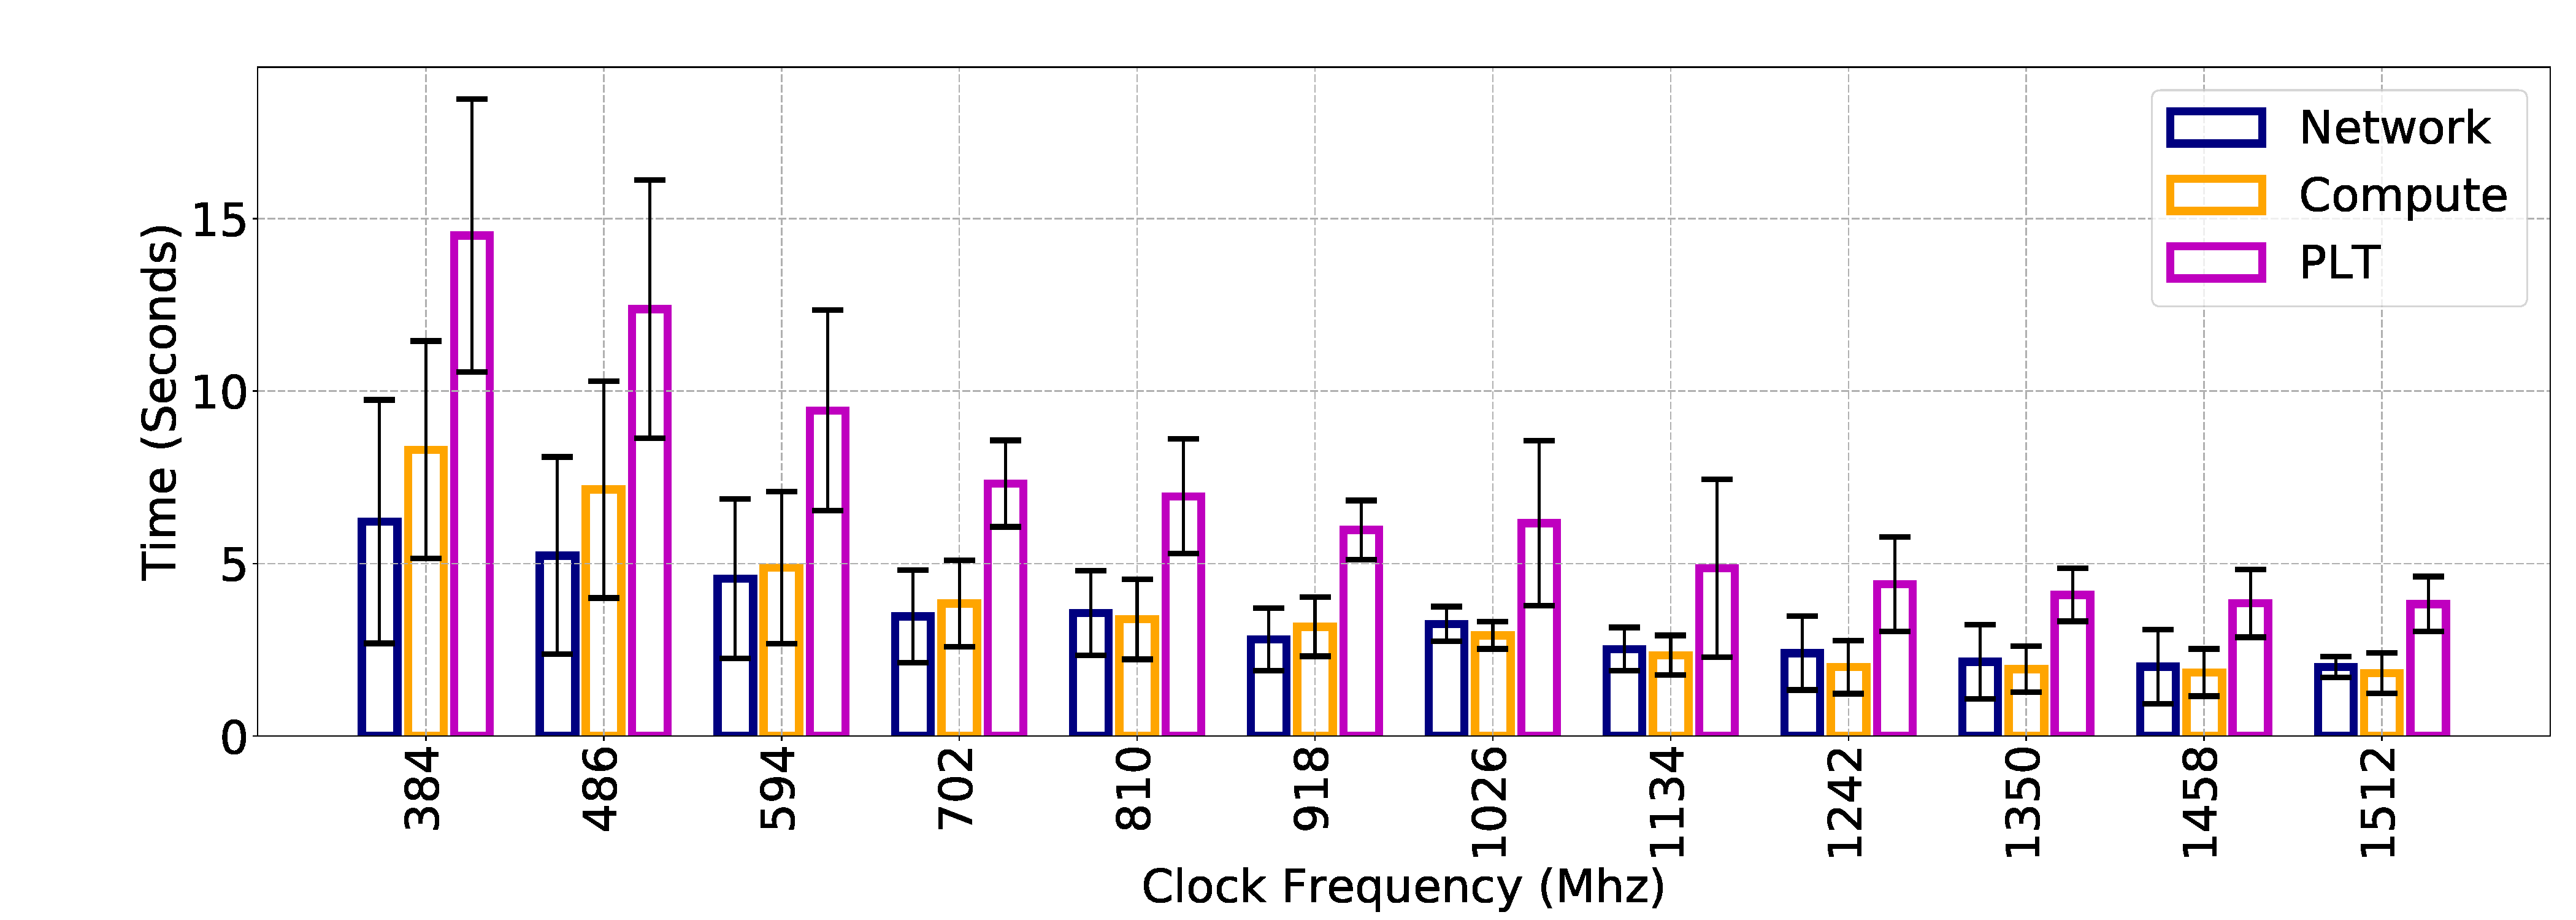
\includegraphics[width=0.8\linewidth]{sections/plt-isolate.pdf}
    \caption{Isolating the effect of network activities and compute activities as the CPU speed changes. The PLT of the Web page is the sum of the time taken for compute activities and the time taken for the network activities on the critical path~\cite{wang2013demystifying,nejati2016depth}. The PLT is the same as that shown in Figure~\ref{fig:plt_clock}. As the CPU slows down, the compute activities are affected more than the network activities. }\vspace{-0.2in}
  \label{fig:plt_isolate}
\end{figure*}

\begin{figure}[t]
  \centering
  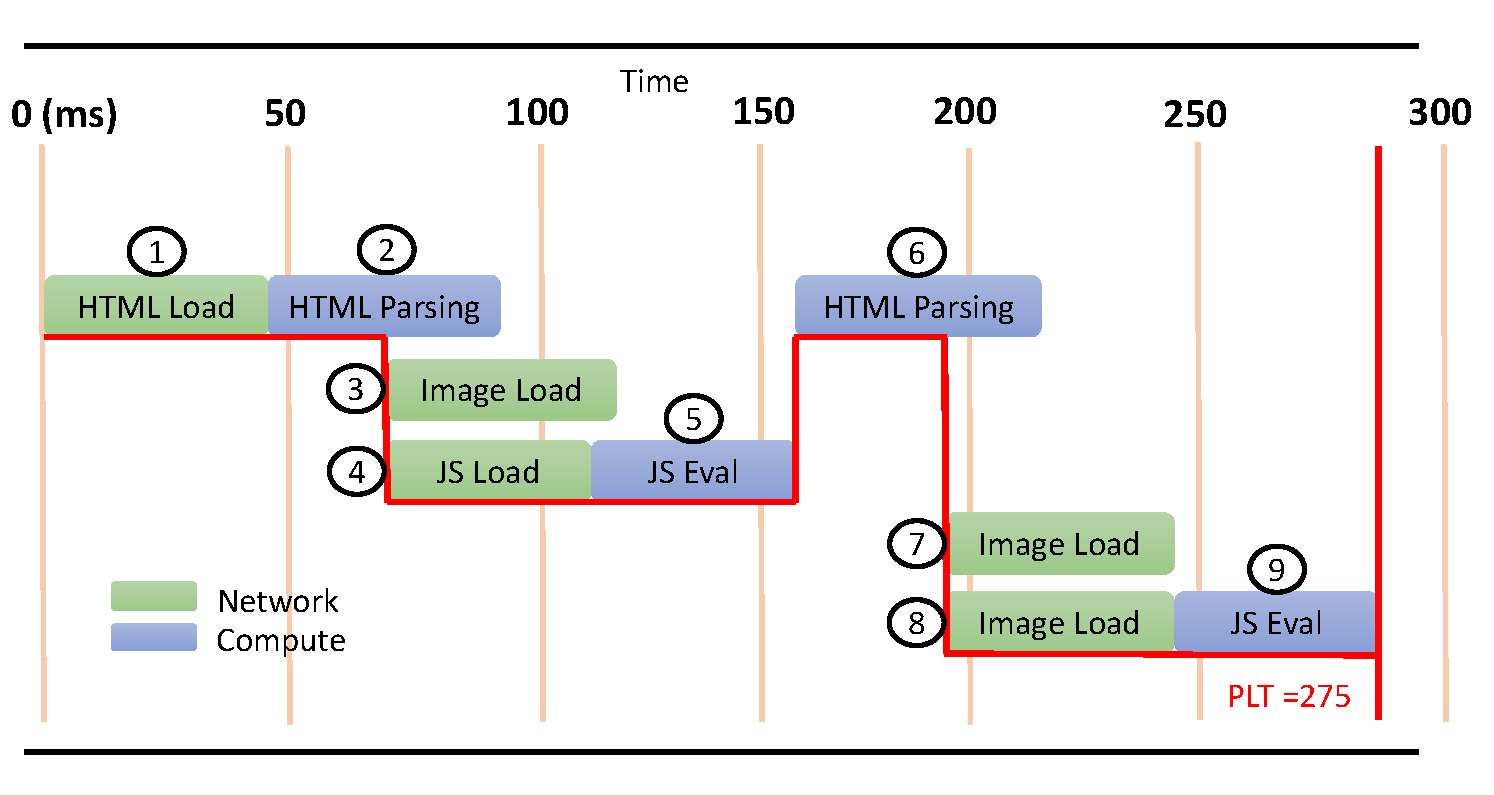
\includegraphics[width=\linewidth]{sections/wprof-dp.pdf}
    \caption{An example page load process divided into its network and compute activities, obtained from the WProf tool~\cite{wang2013demystifying,nejati2016depth}. The red line shows the critical path during the page load process, and represents the page load time. }
  \label{fig:wprof-dp}
\end{figure}

Different from our earlier experiments (\S\ref{sec:motivation}) which were conducted across devices, in this section we study Web QoE  across 12 different CPU speeds on the same device. The experiments are repeated over three smartphones---Nexus 4, Intex Amaze+, and Google Pixel 2 (see Table~\ref{tab:device_types} for specs). The experiments involve loading the top 50 Websites from the Alexa suite~\cite{alexa}.  We use the 
same experimental set up as described in \S\ref{sec:setup}. The CPU speeds are changed using the governor~\cite{ad-governors}. We present the results from Nexus\,4 in detail and summarize the results from the other two phones for brevity.
%
Recall that the Web pages are hosted in a local server and accessed via a well-provisioned LAN so that the performance is not affected by the external network conditions. 

%Web browsing is more complex ecosystem than video applications because of its complex inter dependencies between network and compute activities. In this sectin, we first show the effect of clock on Web QoE and then explain the isolation of clock effect on network and compute. We load the top 50 Web pages from the Alexa list of top 50 Web sites and measure PLT using the setup described in \S\ref{sec:motivation}.

Figure \ref{fig:plt_clock} shows the average PLT across different CPU clock frequencies. The PLT increases 77\% when the CPU clock frequency drops from 1512\,MHz to 384\,MHz. The trends are similar to Figure~\ref{fig:motivation}a where the page loads much slower on low-end devices compared to higher-end devices. In other words, the performance of Web page loads on low-end devices is similar to that of a slower clock on a high-end device. 

\begin{figure}[t]
  \centering
  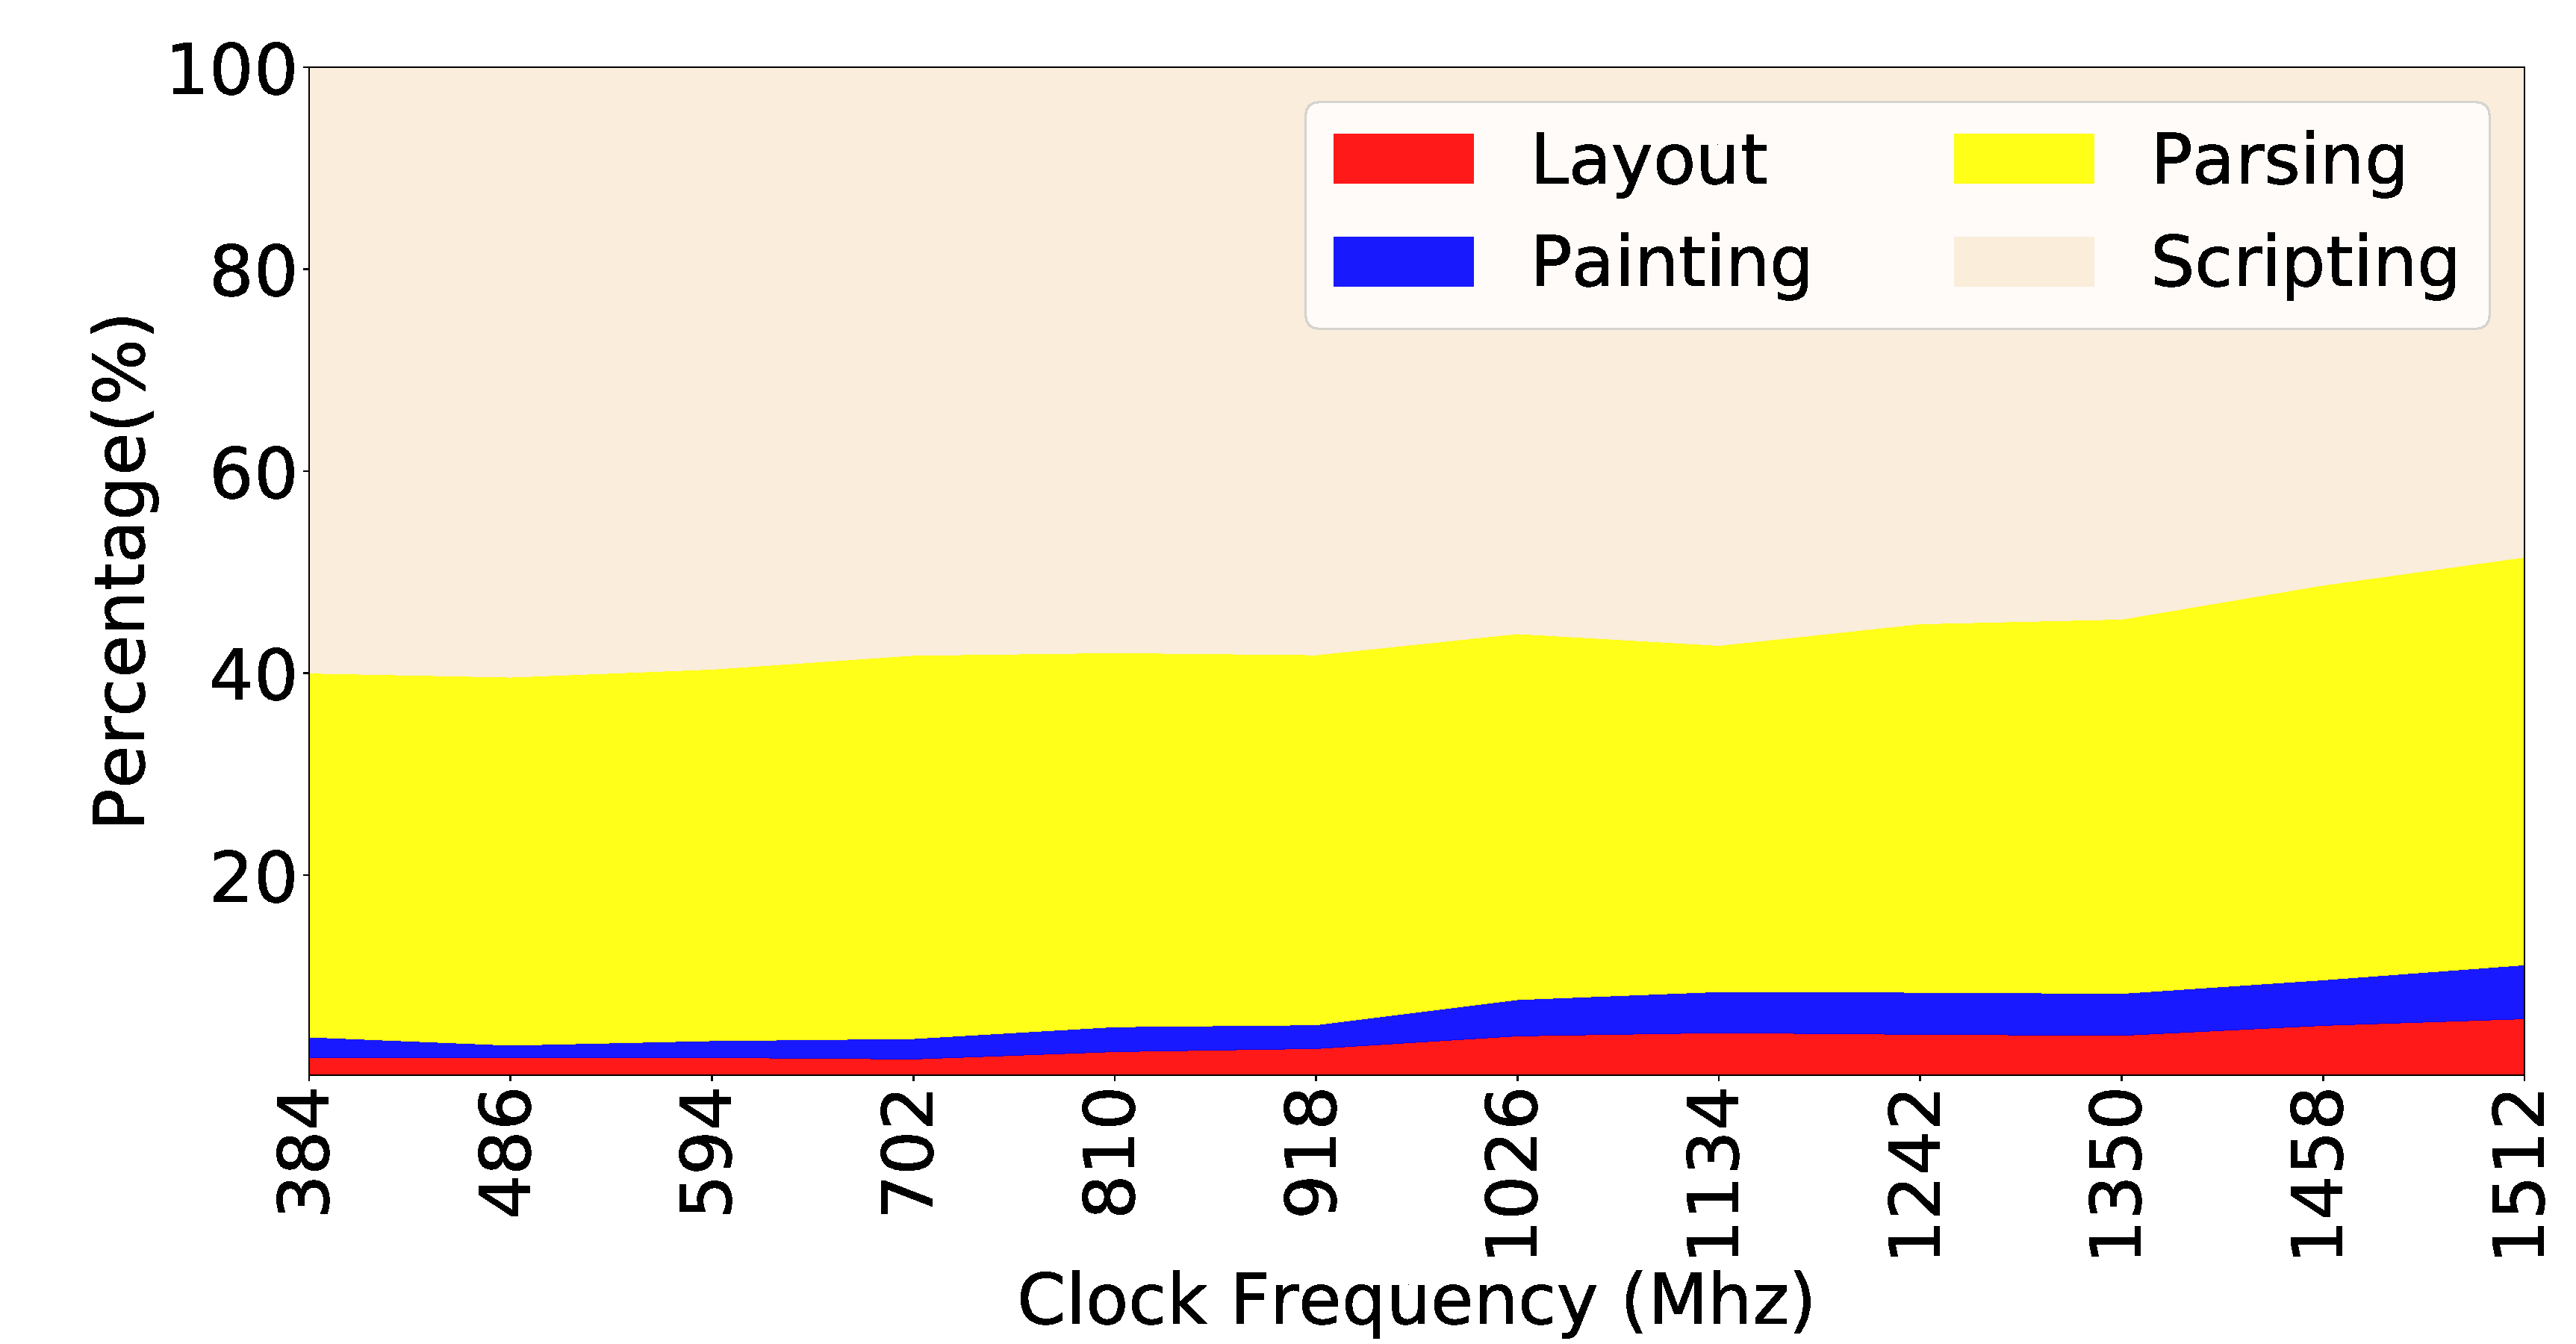
\includegraphics[width=\linewidth]{sections/plt-pie}
  \caption{The time spent on compute activities during page load is further divided into individual activities---Scripting (or Javascript evaluation), HTML Parsing, Layout, and Painting. The scripting time increases significantly when the CPU slows down.  }
  \label{fig:dissect}
\end{figure}

\begin{figure}[t]
  \centering
  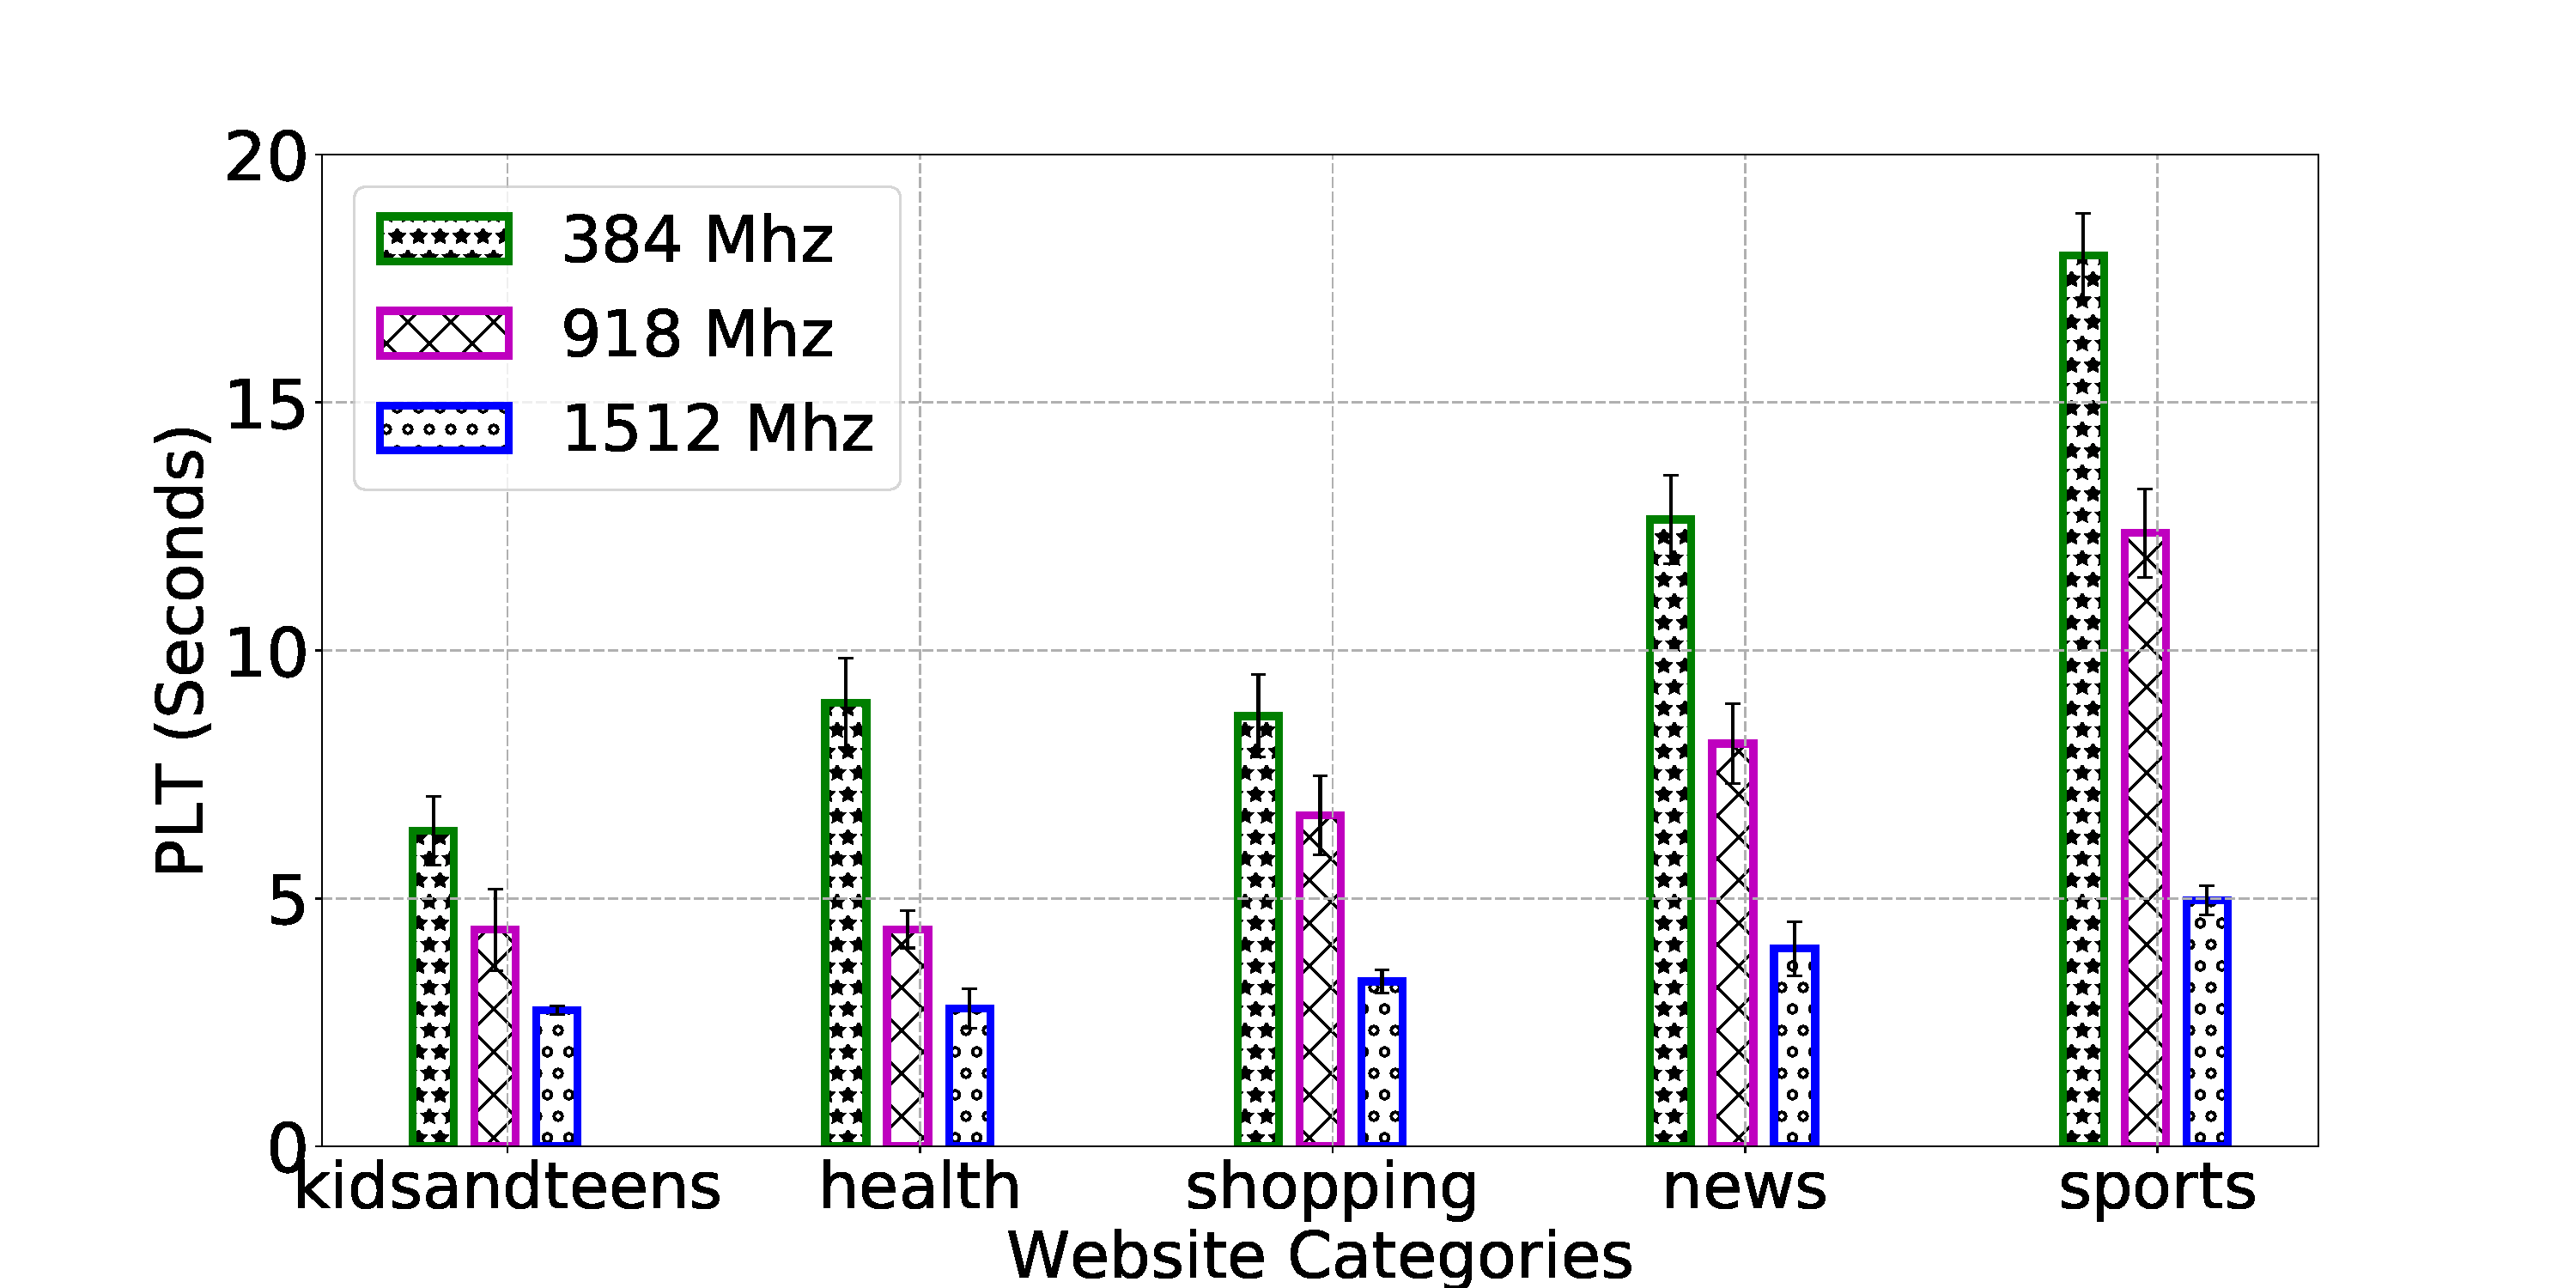
\includegraphics[width=\linewidth]{sections/sites-effect}
  \caption{PLT for three different CPU frequencies for different Webpage categories. The sports Webpages are Javascript-heavy and are affected the most by the CPU 
  slow down.    }
  \vspace{-0.2in}
  \label{fig:sites-effect}
\end{figure}

{\noindent \bf Impact of Network Vs. Compute:}
Our goal now is to determine if the poor Web QoE is because the network throughput drops under slow CPU speeds or  because of slower processing. Recall that the slow CPU speeds not only affects compute but also the network throughput due to the packet processing delays (\S\ref{label:throughput}). The problem is that during Web page loads, network and compute activities are interspersed, making it hard to cleanly separate the effect of network and compute. 
 
 \begin{figure*}[h]
  \subfloat[]{%
  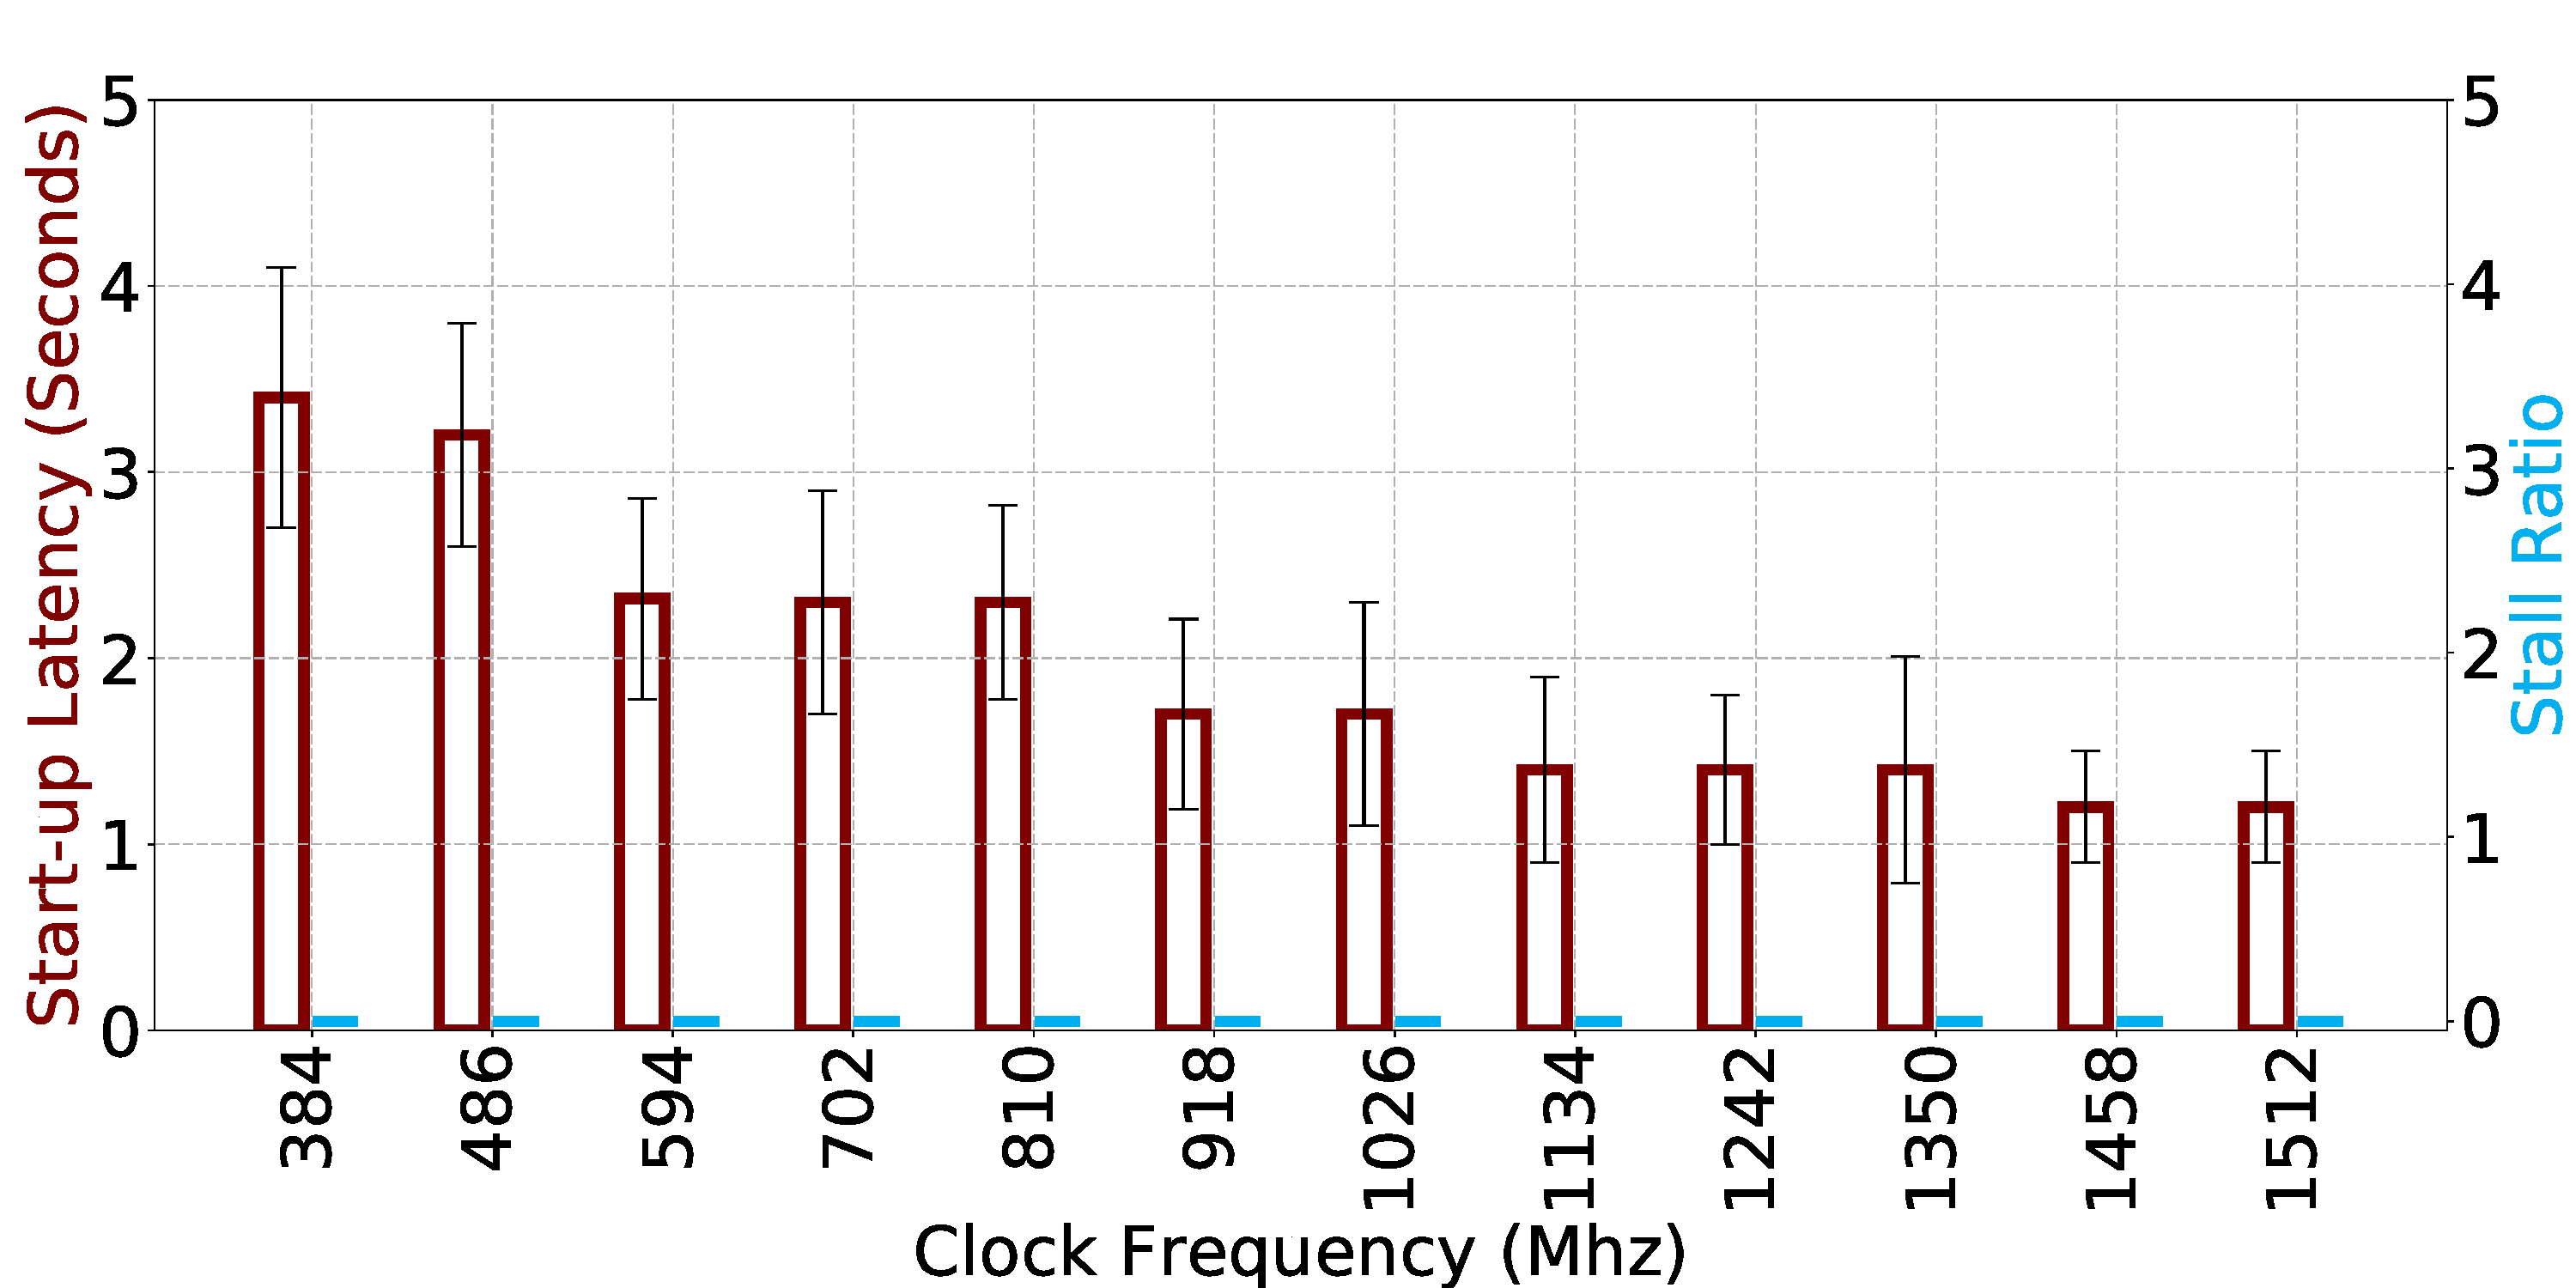
\includegraphics[width=0.5\textwidth]{sections/youtube-clock}
     }
     \subfloat[]{%
  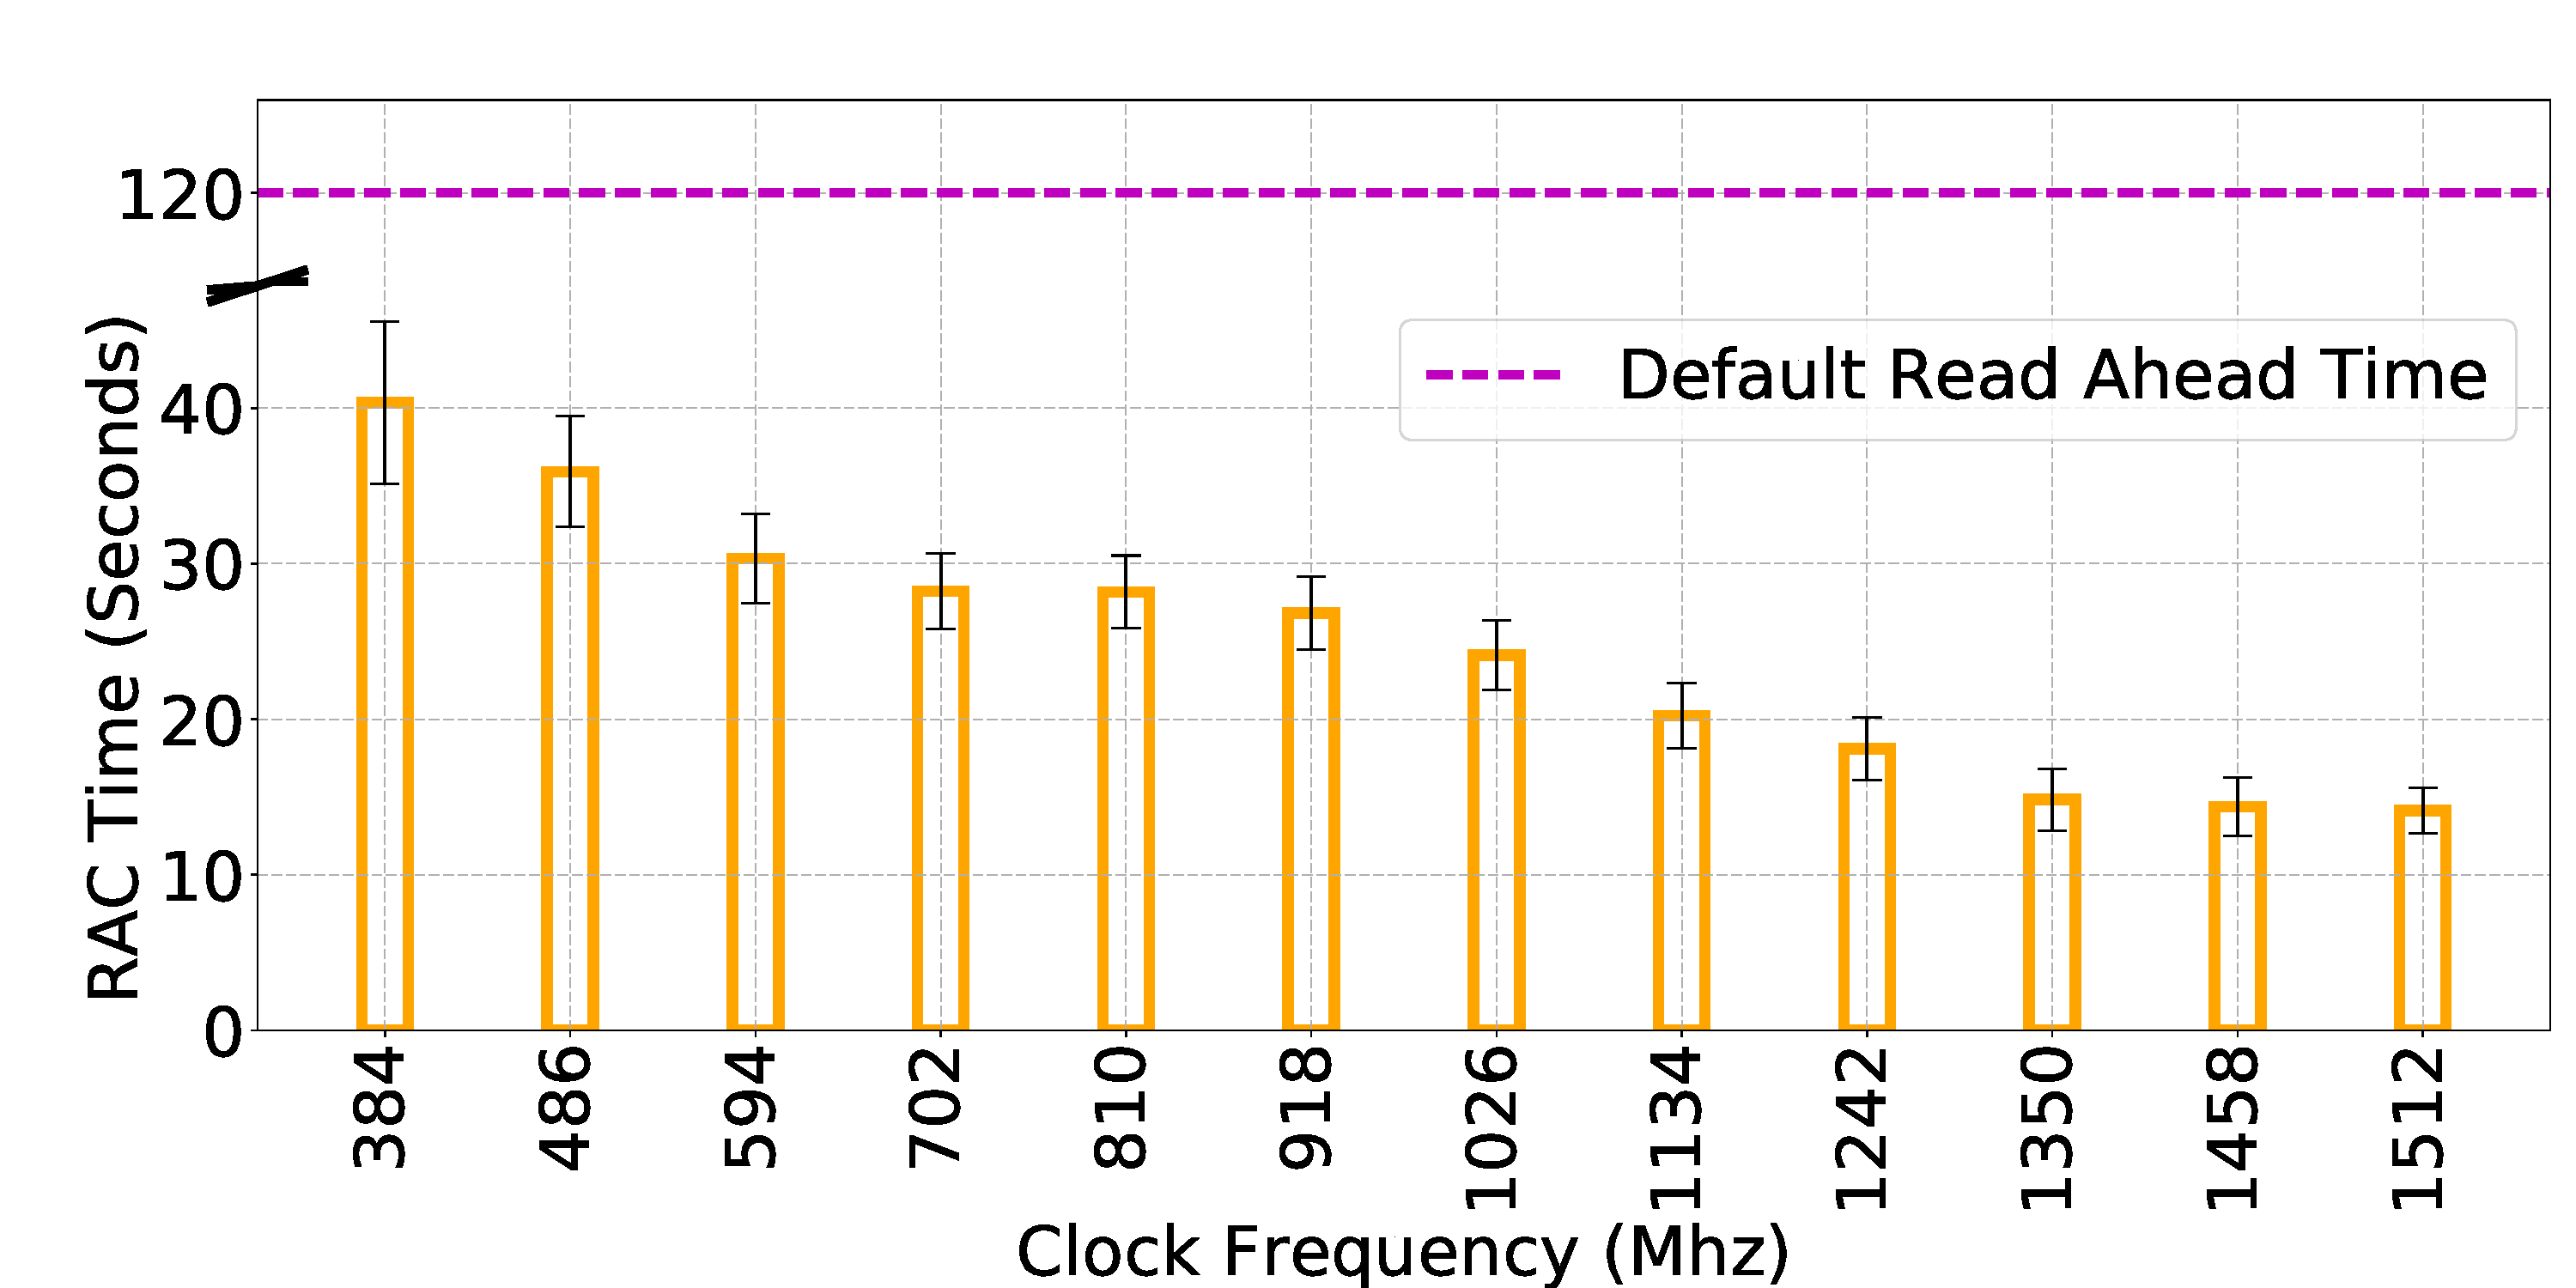
\includegraphics[width=0.5\textwidth]{sections/youtube-rac}
     }
    \caption{(a) Effect of CPU speeds on YouTube: The start-up latency is increased by 50\% but the stall ratio is not affected by the slow clock across the 12 CPU speeds. (b) Isolating the effect of network on stall ratio: The read-ahead convergence time (RAC) is the time required for YouTube to prefetch a read-ahead buffer worth of data (typically 120 seconds of video content). Even under slow clock, the time it takes to prefetch content is well below 120 seconds, which is the time it takes to play the content. As a result, read-ahead buffer is always full and the user does not experience stalls. }
   \vspace{-0.2in}
  \label{fig:youtube}
\end{figure*}

 
Instead, we leverage the WProf tool that extracts the timings of the network and compute activities of the page load process. Figure~\ref{fig:wprof-dp} shows the output provided by the WProf tool~\cite{wang2013demystifying,nejati2016depth} when loading an example page. In this example, the network components are shown in {\em green} and the compute components are shown in {\em blue}. WProf~\cite{wang2013demystifying} (and the version for mobile browsers, WProf-M~\cite{nejati2016depth}) first identifies the timing of each activity. WProf then extracts the dependencies between the activities and draws the dependency graph. For example, in Figure~\ref{fig:wprof-dp}, HTML parsing (6) cannot start until the Javascript (JS) is evaluated (5) because of dependencies between parsing and Javascript evaluation.  The critical path is the bottleneck path in the dependency graph (shown using the red line); the length of the critical path provides the PLT. %As the CPU speeds change, the dependency graph and the critical path change, making it hard to isolate the effect of network and compute.

Using WProf, we estimate the time on the critical path involving compute activities (HTML parsing, scripting, rendering, and CSS evaluation) and network activities (object loading) as shown in Figure~\ref{fig:plt_isolate}. The sum of the network and compute activities gives the PLT (the PLT numbers are from Figure~\ref{fig:plt_clock}). The network time on the critical path increases from an average of 2 seconds when the clock speed is 1512\,MHz to 6 seconds when the clock speed is increased to 384\,MHz -- a 66\% increase. The compute time increases by 76\% for the same CPU slow down. We find that the compute time increases even more compared to network time for more complex Webpages (not shown here). 

%The key takeaway is that for Web applications, processing the Web page takes a bigger hit under slow CPU conditions compared to network, although the effect of slow CPU on network is still significant.
%\noindent \textbf{PLT Breakdown}: 
Figure~\ref{fig:dissect} further dissects the compute activities into HTML parsing, JS scripting, CSS evaluation, layout and painting. 
%We measure the fraction of time spent on these activities individually using WProf tool. 
Scripting times increase the most as the CPU clock slows down; it accounts for 51\% of the overall compute times at high CPU frequencies, and 60\% at low CPU frequencies. The layout and painting only account for 4\% of the compute time on the critical path. 

The  takeaway from Figure~\ref{fig:dissect} is that, a key component for improving Web page loads, especially at slow CPU speeds, is to  improve the efficiency of scripting. 
%
Figure~\ref{fig:sites-effect} demonstrates
this in another way -- Websites with a large number of Javascript are affected the most when the CPU slows down. In this experiment, we choose the top 50 pages from the  Alexa suite~\cite{alexa} under different categories -- kids and teen, health, shopping, news, and sports. 
%The categories are ordered according to the time spent on scripting/Javascript evaluation when the phone is operating at 1512\,MHz. 
The sports Webpages spend the most time on scripting and clearly suffers the maximum slow down (up to 13\,sec) when CPU frequency drops from the fastest
to the slowest. On the other hand, kids and teen Webpages increases by $<3.5$ seconds. We leverage this observation to improve Web page load performance (\S\ref{label:whatif}).

%As the CPU speeds reduces, Webpages with more scripting is affected more compared to the other Webpages. The average PLT for the Webpages categorized under sports and news increases by 13 and 9 seconds respectively when the CPU speed decreases. On the other hand, Webpages under the kids and teens category increases by less than 3.5 seconds. We leverage this observation to improve Web page load performance (\S\ref{label:whatif}).

 %To see this effect, we measure PLT for different categories of websites from Alexa website. Sports websites have 52\% scripting, the largest among the different categories. As a result, the PLT of sports Websites are most affected by slowing down the CPU compared to other categories. 

%To this end, we write an emulator; the emulator replays the page load process under different CPU frequencies and loads network objects as before, but assumes that the compute time remains a constant. This is of course not the case since change CPU frequencies will change compute. However, the goal of the emulator is to isolate the effect of CPU speed on the network loading alone~\footnote{The source code of the emulator is uploaded at this website: \url{https://github.com/SantiagoVargas/PALO}}


%shows the effect of clock frequency on PLT. 
%We observe 77\% increase in PLT from high clock to low clock. This is most observed impact of clock
%We note that at low frequencies below $594Mhz$, the PLT reduces sharply with an increase in frequency. 
%From $594Mhz$ to $1512Mhz$, the page load reduces in a linear fashion. 

%We now explain the faster than linear improvement with an increase in clock speed of PLT. 
%We note that the PLT depends on two distinct factors -- loading, which depends on packet processing and parsing, which depends on computation. 
%As shown in \S\ref{label:throughput}, packet processing also slows down with a slower clock frequency. 
%Since packet processing and loading are interdependent on each other, a faster CPU clock leads to improvement in both and thus a faster than linear improvement in the overall PLT.

%We also plot the effect of CPU load on PLT at different loads for three different frequencies ($384 MHz$, $918 MHz$ and $1512 MHz$). We observe that at a frequency of $1512 MHz$, the CPU load only affects the PLT by a maximum of $1s$. However, at $384 MHz$, the PLT increases by over $8s$ when the load increases from $0\%$ to $100\%$. Moreover, the increase in the CPU load leads to a super-linear increase in the PLT. For example, at $384 MHz$, the PLT increases by only $2s$ when we change the CPU load from $0\%$ to $50\%$, whereas it increases by over $6s$ for that of $50\%$ to $100\%$.

%\begin{figure}[t]
%  \centering
%  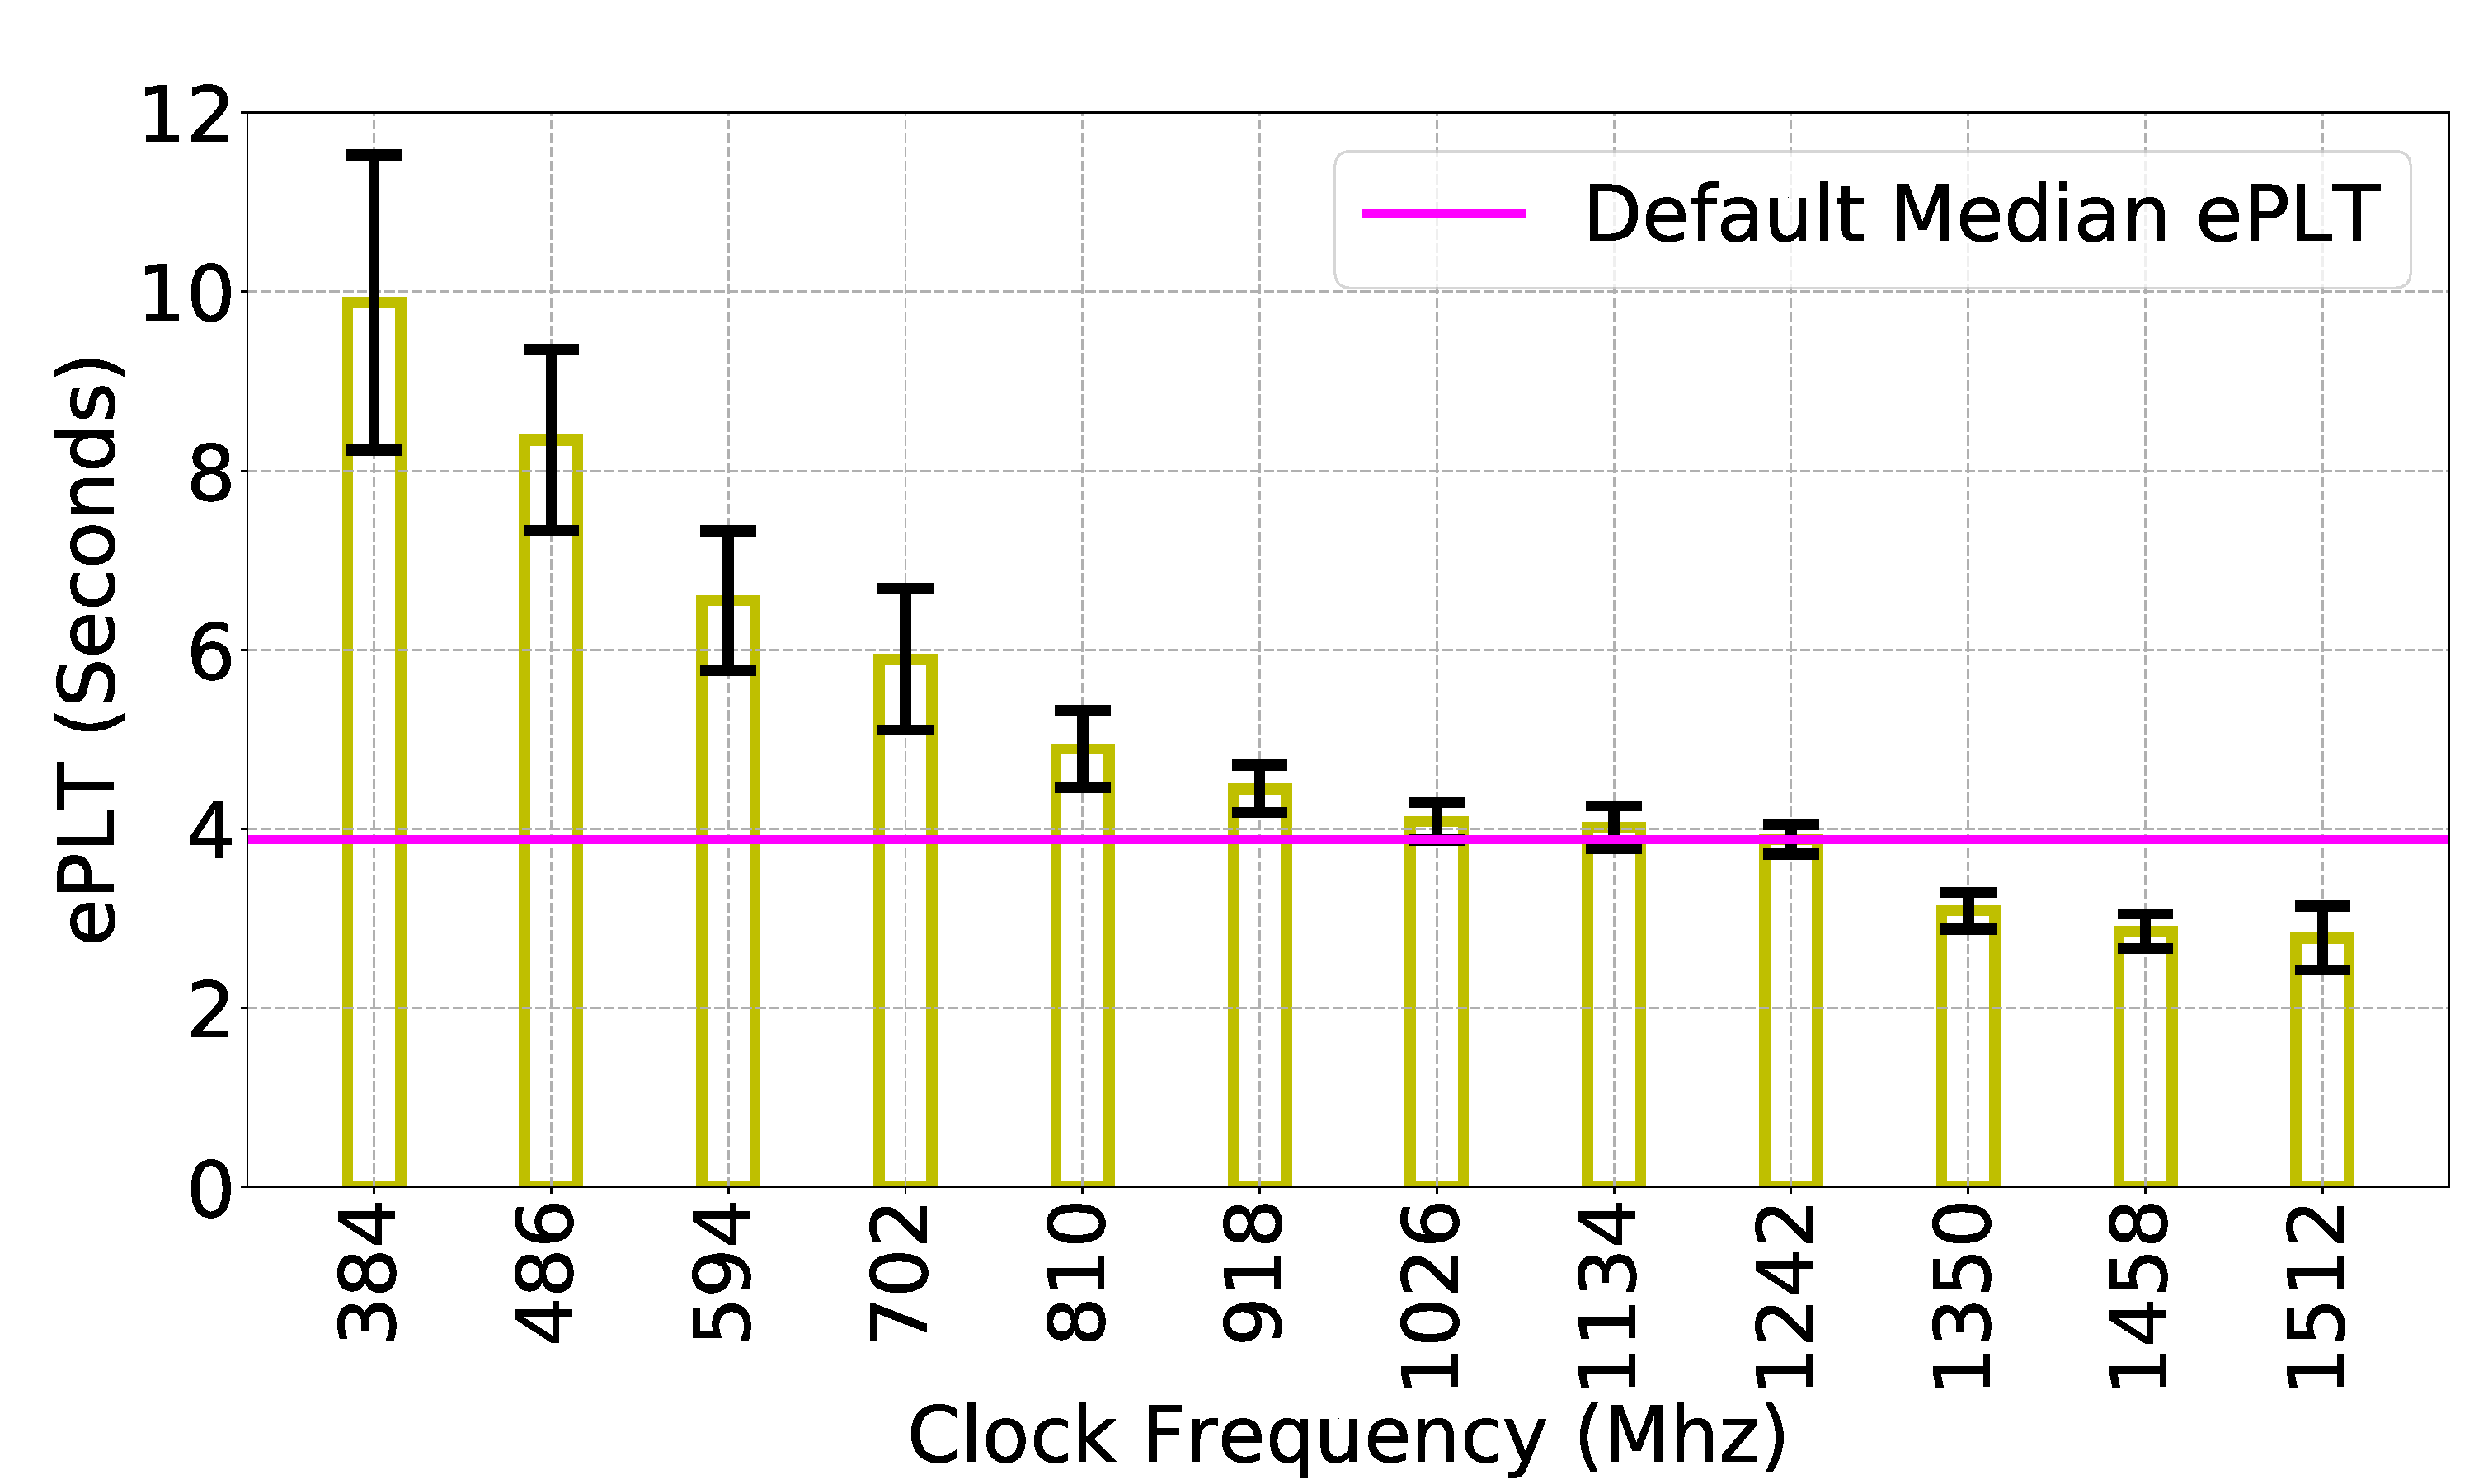
\includegraphics[width=\linewidth]{sections/eplt}
%    \caption{\textit{Emulated Page loads using WProf dependency graph. The \textit{ePLT} is increased by 7 seconds at lower clock and gradually decreased with the increased clock from 594Mhz.}}
%  \label{fig:eplt}
%\end{figure}

%\noindent\textbf{Network} 

%To isolate the impact of clock on network during page load, we need to preserve the dependencies and computation of real pages. 

%Figure~\ref{fig:emulator} shows the 

%This allows us to schedule live object downloads during the page load and maintain a fixed, simplified computation. 
%We record the page load process by capturing the dependency graph with WProf \cite{wang2013demystifying}. 
%WProf preserves the dependency and computation timing information during the page load. 
%We replay the page load process using recorded dependency graph as input to the emulator.
%
%To see the effect of clock frequency on network performance, the web page emulator processes the web page dependency information as does a normal browser, excluding the activities of rendering and painting which are negligible on PLT. 
%Using the dependency information obtained earlier, all page load activities are modeled as a DAG such that there are child activities which are dependent upon multiple parent activities that must first finish execution before the child activity begins its execution. 
%The entire scheduling process is concurrent in that multiple activities are scheduled to run at the same time. 
%In general there are two types of dependencies, direct dependencies which are scheduled to run as soon as a parent dependency finishes its execution and timed dependencies which are scheduled after a certain amount of time relative to the start of their parent activity. 
%The emulation process starts by first executing the main activity, a network request of the main HTML file of the web page being requested. 
%The entire emulation process is timed, and the total time taken is reported as the \textit{emulated PLT (ePLT)}.

%We measure \textit{ePLT} as the time it takes to load the page in the emulator. % to understand the impact of page computation and dependencies. We implement the \textit{ePLT} emulator using client-side Javascript in webpage. We host the recorded webpage (a JSON file with dependecy information) on a Node.js server in our LAN. We load our emulator webpage on Nexus4 phone Chrome browser and measure the \textit{ePLT} by varying clock. 
%Figure \ref{fig:eplt} shows the impact of clock on \textit{ePLT}. 
%The default \textit{ePLT} is the \textit{ePLT} with no fixed clock i.e, under default \texttt{OD} frequency governor which changes the clock dynamically based on the need. 
%The default median \textit{ePLT} is 3.88 seconds, which is 0.9 seconds less than the best possible \textit{ePLT} under 1512Mhz clock. 
%It becomes far worse (10 seconds) under slow clock. This tells that there is a significant impact ($>43$\% of original PLT) of clock on downloading objects due to packet processing delays.  \\
%\begin{figure}[t]
%  \centering
%  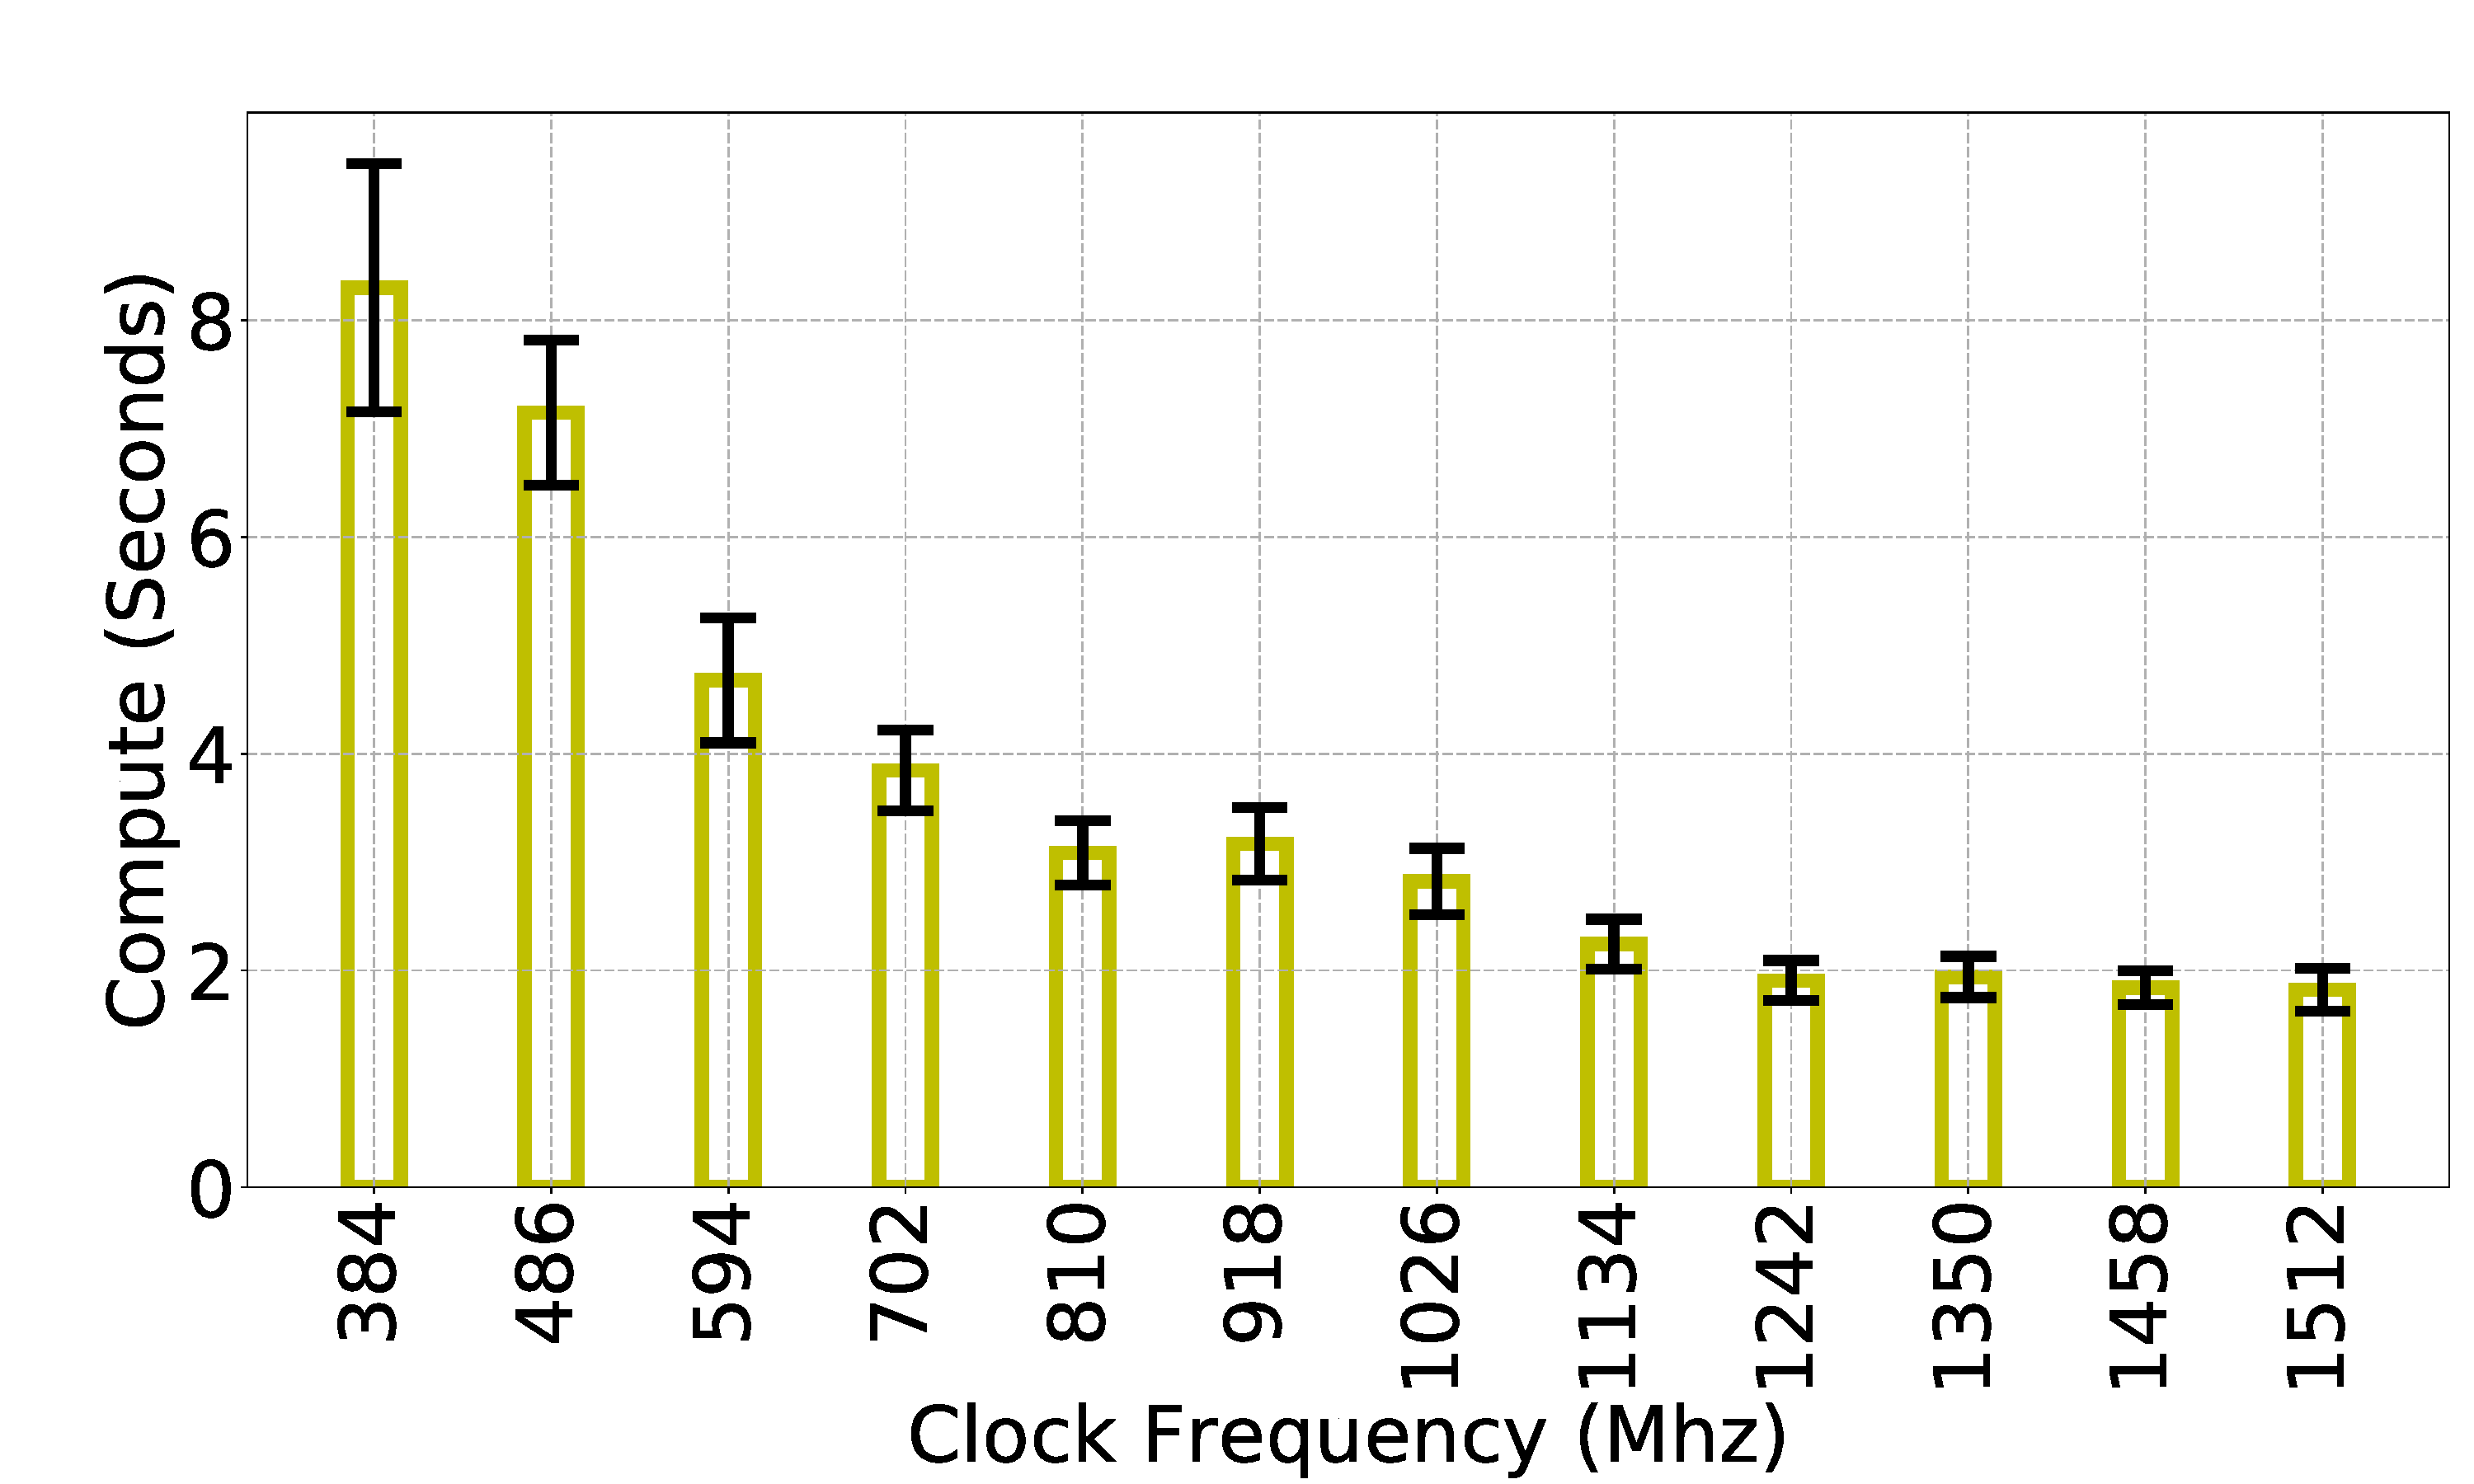
\includegraphics[width=\linewidth]{sections/compute-plt.pdf}
%  \caption{\textit{Effect of clock on compute activities during page load.}}
%  \label{fig:compute}
%\end{figure}

%\noindent \textbf{Compute Isolation:} 
%We use Wprof tool to isolate the compute effect of clock. 
%WProf gives the time spent different compute activites during a page load. 
%We take the sum of time spent on scripting, parsing, layout and painting as compute time.
%Figure \ref{fig:compute} shows the effect of clock on only compute activities. 
%We observe more than 6 seconds of PLT increase from high clock to low clock. 
